\documentclass[handout]{beamer}

\setbeamercovered{dynamic}
\usetheme{Marburg}
\setbeamertemplate{navigation symbols}{} 
\setbeamertemplate{footline}
{
  \leavevmode%
  \hbox{%
  \begin{beamercolorbox}[wd=.333333\paperwidth,ht=2.25ex,dp=1ex,center]{author in head/foot}%
    \usebeamerfont{author in head/foot}\copyright $\ $ \insertshortauthor%~~\beamer@ifempty{\insertshortinstitute}{}{(\insertshortinstitute)}
  \end{beamercolorbox}%
  \begin{beamercolorbox}[wd=.333333\paperwidth,ht=2.25ex,dp=1ex,center]{title in head/foot}%
    \usebeamerfont{title in head/foot} Iowa State University
  \end{beamercolorbox}%
  \begin{beamercolorbox}[wd=.333333\paperwidth,ht=2.25ex,dp=1ex,right]{date in head/foot}%
    \usebeamerfont{date in head/foot}\insertshortdate{}\hspace*{2em}
    \insertframenumber{} / \inserttotalframenumber\hspace*{2ex} 
  \end{beamercolorbox}}%
  \vskip0pt%
}

\usepackage{amsmath}
%\usepackage{caption}
\usepackage{color}
\usepackage{enumerate}
\usepackage{listings}
\usepackage{hyperref}
\usepackage{mathrsfs}
\usepackage{natbib}
\usepackage{url}

\providecommand{\all}{\ \forall \ }
\providecommand{\bs}{\backslash}
\providecommand{\e}{\varepsilon}
\providecommand{\E}{\ \exists \ }
\providecommand{\lm}[2]{\lim_{#1 \rightarrow #2}}
\providecommand{\m}[1]{\mathbb{#1}}
\providecommand{\nv}{{}^{-1}}
\providecommand{\ov}[1]{\overline{#1}}
\providecommand{\p}{\newpage}
\providecommand{\q}{$\quad$ \newline}
\providecommand{\rt}{\rightarrow}
\providecommand{\Rt}{\Rightarrow}
\providecommand{\vc}[1]{\boldsymbol{#1}}
\providecommand{\wh}[1]{\widehat{#1}}

\hypersetup{colorlinks,linkcolor=,urlcolor=blue}
\numberwithin{equation}{section}

\definecolor{dkgreen}{rgb}{0,0.6,0}
\definecolor{gray}{rgb}{0.5,0.5,0.5}
\definecolor{mauve}{rgb}{0.58,0,0.82}

\lstset{ 
  language=C,                % the language of the code
  basicstyle= \footnotesize,           % the size of the fonts that are used for the code
  numberstyle= \tiny \color{white},  % the style that is used for the line-numbers
  stepnumber=2,                   % the step between two line-numbers. 
  numbersep=5pt,                  % how far the line-numbers are from the code
  backgroundcolor=\color{white},      % choose the background color. You must add \usepackage{color}
  showspaces=false,               % show spaces adding particular underscores
  showstringspaces=false,         % underline spaces within strings
  showtabs=false,                 % show tabs within strings adding particular underscores
  frame=lrb,                   % adds a frame around the code
  rulecolor=\color{black},        % if not set, the frame-color may be changed on line-breaks within not-black text 
  tabsize=2,                      % sets default tabsize to 2 spaces
  captionpos=t,                   % sets the caption-position 
  breaklines=true,                % sets automatic line breaking
  breakatwhitespace=false,        % sets if automatic breaks should only happen at whitespace
  %title=\lstname,                   % show the filename of files included with \lstinputlisting;
  keywordstyle=\color{blue},          % keyword style
  commentstyle=\color{gray},       % comment style
  stringstyle=\color{dkgreen},         % string literal style
  escapeinside={\%*}{*)},            % if you want to add LaTeX within your code
  morekeywords={*, ...},               % if you want to add more keywords to the set
  xleftmargin=0.053in, % left horizontal offset of caption box
  xrightmargin=-.03in % right horizontal offset of caption box
}

%\DeclareCaptionFont{white}{\color{white}}
%\DeclareCaptionFormat{listing}{\parbox{\textwidth}{\colorbox{gray}{\parbox{\textwidth}{#1#2#3}}\vskip-0.05in}}
%\captionsetup[lstlisting]{format = listing, labelfont = white, textfont = white}
%For caption-free listings, comment out the 3 lines above and uncomment the 2 lines below.
 %\captionsetup{labelformat = empty, labelsep = none}
 %\lstset{frame = single}

\title{Dispersion Estimation and Its Effect on Test Performance in RNA-seq Data Analysis}
\author{Will Landau \\ Dr. Peng Liu}
\date{March 1, 2013}

\begin{document}

\begin{frame}
\titlepage
 \end{frame}
 
 \AtBeginSection[]
{
   \begin{frame}
       \frametitle{Outline}
       \tableofcontents[currentsection]
   \end{frame}
}


\section{Background}

\begin{frame}
\frametitle{}
\setkeys{Gin}{height=.8\textheight}
\setkeys{Gin}{width=1\textwidth}
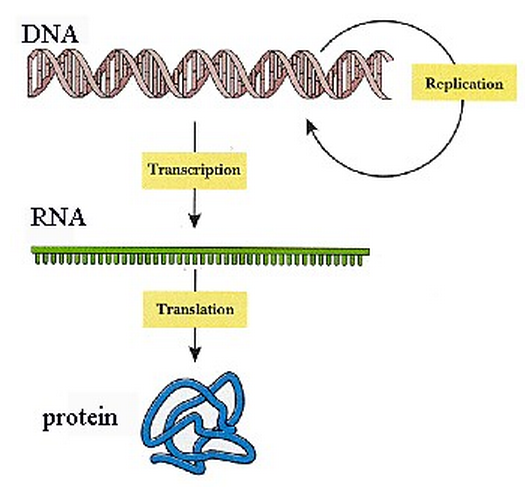
\includegraphics{../fig_perm/transc.png}
\end{frame}



\begin{frame}
\frametitle{Next Generation Sequencing (NGS) Technologies} \small
\begin{itemize}
\pause \item A NGS platform measures the relative abundance of each RNA sequence in a sample. 
\pause \item Example: Illumina's Genome Analyzer.
\end{itemize}

\setkeys{Gin}{height=.45\textheight}
\setkeys{Gin}{width=.45\textwidth}
\begin{center}
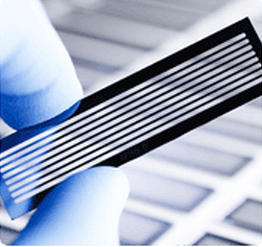
\includegraphics{../fig_perm/flowcell.png} $\ $ 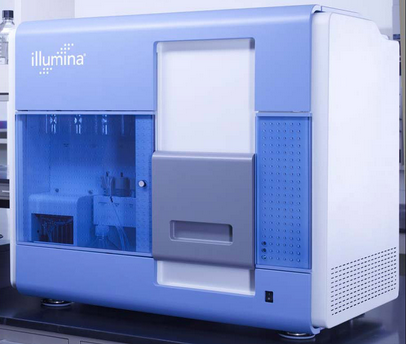
\includegraphics{../fig_perm/illumina.png}
\end{center}
\end{frame}

\begin{frame}
\frametitle{RNA-Seq Workflow}
\setkeys{Gin}{width=1\textwidth}
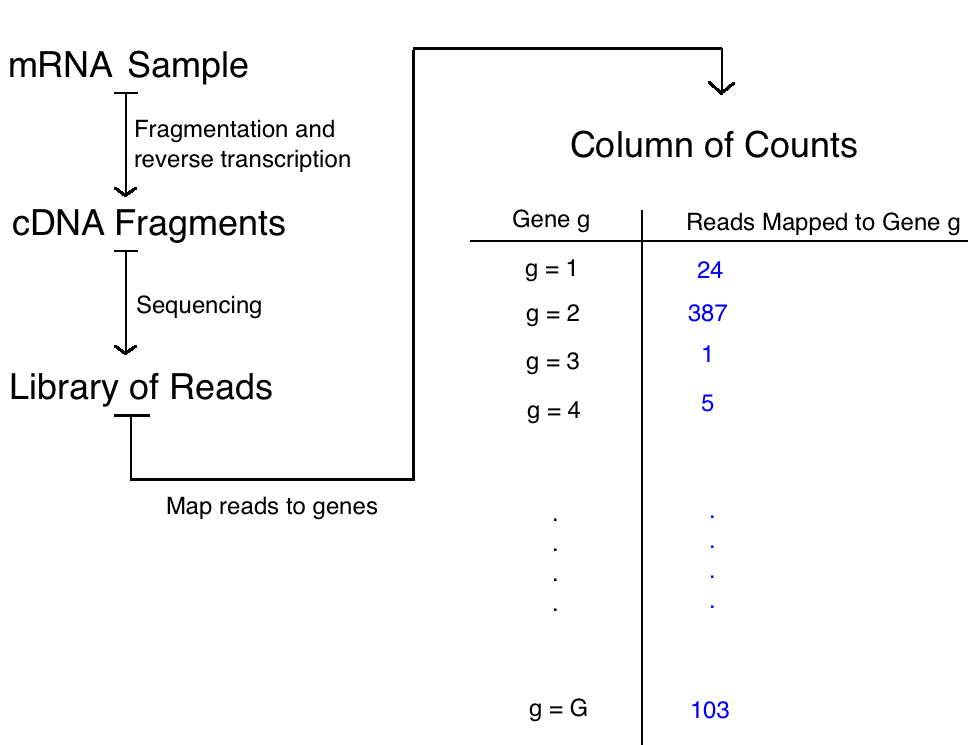
\includegraphics{../fig_perm/workflow.png}
\end{frame}



\begin{frame}
\frametitle{RNA-Seq Experiments}
\begin{itemize}
\pause \item Sequence multiple RNA samples from two or more treatment groups. 
\begin{itemize}
\pause \item Biological replicates: original samples of genetic material (experimental units).
\pause \item Technical replicates: repeated sequencing trials of the same sample of genetic material (observational units).
\begin{itemize}
\pause \item Libraries from different technical replicates may be pooled within each biological replicate.
\end{itemize}
\end{itemize}
\pause \item Central question: \emph{which genes are differentially expressed across treatment conditions?}
\end{itemize}
\end{frame}


\begin{frame}
\frametitle{An RNA-Seq Dataset}
\setkeys{Gin}{width=1\textwidth}
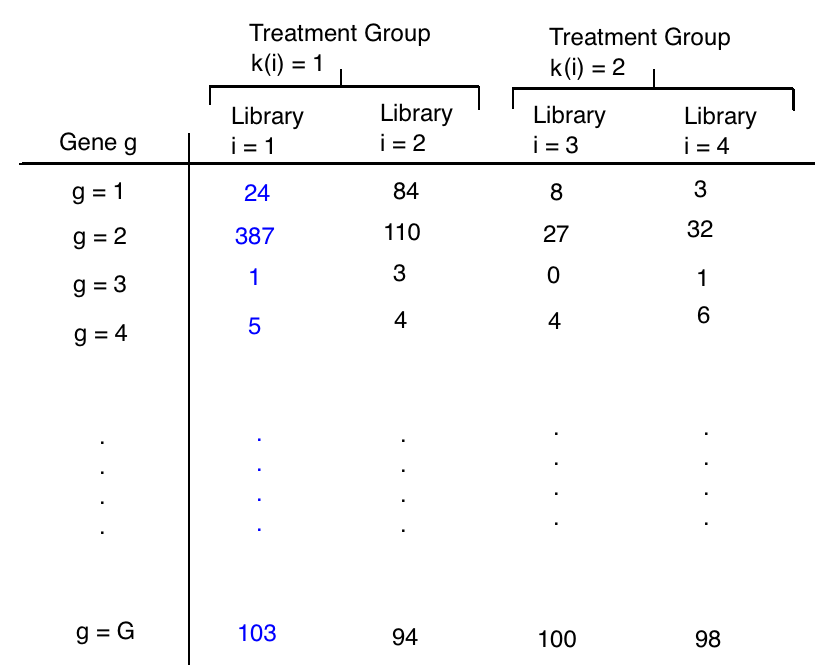
\includegraphics{../fig_perm/data.png}
\end{frame}


\begin{frame}
\frametitle{The Negative Binomial Model}

\begin{itemize}
\pause \item Let $Y_{g, i}$ be the number of reads in library $i$ mapped to gene $g$.
\pause \item If $Y_{g, i} \sim$ NB($\mu_{g, i}$, $\phi_g$), then:
\end{itemize}

\scriptsize
\pause \begin{align*} 
f(y \mid \mu_{g, i}, \phi_g) &= \frac{\Gamma(y+ \phi_g \nv)}{\Gamma(\phi_g \nv) \Gamma(y + 1)} \left ( \frac{\phi_g \nv}{\mu_{g, i} + \phi_g \nv} \right ) ^{\phi_g \nv} \left ( 1 - \frac{\phi_g \nv}{\mu_{g, i} + \phi_g \nv} \right )^ {y} \\ \nonumber \\
\end{align*}
\normalsize

\begin{itemize}
\pause \item As $\phi_g \rt 0$, $f$ converges to the Poisson pmf.
\pause \item $\text{Var}(Y_{g, i}) = \mu_{g, i} + \mu_{g, i}^2 \phi_g$
\pause \item $E(Y_{g, i}) = \mu_{g, i} = s_i \cdot \nu_{g, k(i)}$, where:
\begin{itemize}
\pause \item $s_i$ is the normalization factor of library $i$.
\pause \item $k(i)$ is the treatment group of library $i$.
\pause \item $\nu_{g, k(i)}$ is the normalized true mean expression level of gene $g$ in the libraries of treatment group $k(i)$.
\end{itemize} 
\end{itemize}


\end{frame}

\begin{frame}
\frametitle{Normalization factors}
\begin{itemize}
\pause \item The normalization factors, $s_i$, account for differences in library sizes caused by different sequencing depths and other technical factors.
\pause \item Si and Liu (2012) show that the following method, proposed by Anders and Huber (2010), performs well:
\pause \begin{align*}
s_i = \text{Median}_g \frac{y_{g, i}}{ \left (\prod_{i = j}^n y_{g, j} \right)^{1/n}}
\end{align*}
\pause where $n$ is the total number of libraries.
\pause \item Note: to avoid dividing by zero, in practice, all zero counts are set to a small constant for this calculation.
\end{itemize}
\end{frame}






\begin{frame}
\frametitle{Objectives}
\begin{itemize}
\pause \item Review current methods for estimating dispersion parameters in negative binomial models for RNA-Seq data
\pause \item Use a simulation study to evaluate and compare the effectiveness of these methods in terms of:
\begin{itemize}
\pause \item Point estimation quality.
\pause \item The performance of tests to detect differentially expressed genes.
\end{itemize}
\end{itemize}
\end{frame}


























\section{Currently Available Methods}

\subsection{Dispersion Estimation}


\subsubsection{QL}


\begin{frame}
\frametitle{\small The quasi-likelihood (QL) method (Robinson and Smyth, 2007)}
\small
\begin{itemize}
\pause \item Implementation: package {\tt AMAP.Seq} (Si and Liu, 2012)
\pause \item Iteratively estimate:
\begin{itemize}
\pause \item The negative binomial MLE, $\wh{\mu}_{g, i}$, of $\mu_{g, i}$, given $\phi_g = \wh{\phi}_g$.
\pause \item $\wh{\phi}_g$, the quasi-likelihood tagwise dispersion estimate given $\mu_{g, i} = \wh{\mu}_{g, i}$, which is calculated by solving for $\wh{\phi_g}$:

\pause \begin{align*}
2 \sum_{i = 1}^n & \left \{ y_{g, i} \log \left [ \frac{y_{g, i}}{\wh{\mu}_{g, i}} \right ] - (y_{g, i} + \wh{\phi}_g \nv) \log \left [ \frac{y_{g, i} + \wh{\phi}_g \nv}{\wh{\mu}_{g, i} + \wh{\phi}_g \nv} \right ] \right \} 
\\ &= n - 1
\end{align*}

\end{itemize}
\end{itemize}

\end{frame}

 
\subsubsection{DSS}


\begin{frame}
\frametitle{\small The dispersion shrinkage for sequencing (DSS) method (Wu, Wang, and Wu, 2012)}
\small

\begin{itemize}
\pause \item Idea: shrink $\wh{\phi}_g$ towards a common \emph{prior} instead of a common value or trend.
\pause \item Decompose the negative binomial into a Poisson-Gamma hierarchical model:
\begin{align*}
\uncover<4->{Y_{g, i} \mid \theta_{g, i}} & \uncover<4->{\sim \text{Poisson}(\theta_{g, i} s_i)} \\
\uncover<5->{\theta_{g, i} \mid \phi_g} & \uncover<5->{\sim \text{Gamma}(\nu_{g, k(i)}, \phi_g)} \\
\uncover<6->{\phi_g} & \uncover<6->{\sim \text{log-normal}(m_0, \tau^2)}
\end{align*}
\pause \pause \pause
\pause \item The marginal distribution of the $Y_{g, i}$'s is NB($\mu_{g, i}, \phi_g$), where $\mu_{g, i} = s_i \nu_{g, k(i)}$ as before.
\pause \item Each $\wh{\phi}_g$ is the mode of the posterior density of $\phi_g$. 
\pause \item Implementation: package {\tt DSS}
\end{itemize}
\end{frame}



\subsubsection{wqCML}

\begin{frame}
\frametitle{\small The weighted quantile-adjusted conditional maximum likelihood (wqCML) method (Robinson \& Smyth, 2007)} \scriptsize

\begin{itemize}
\pause \item Implementation:
\begin{itemize}
\pause \item \scriptsize Package {\tt edgeR}.
\pause \item \scriptsize Use the {\tt estimateTagwiseDisp()} function.
\pause \item \scriptsize Optionally, set $\alpha$ with the {\tt prior.n} argument.
\end{itemize}

\pause \item Maximize the weighted log likelihood:

\pause \begin{align*}
\text{WLL}(\phi_g) = l_g(\phi_g) + \alpha l_C(\phi_g)
\end{align*}

\begin{itemize}
\pause \item \scriptsize $l_C$: the ``common" log likelihood, the negative binomial log likelihood under the restriction that all genes share the same dispersion value.
\pause \item \scriptsize $l_g$: the log likelihood used in the quantile-adjusted conditional maximum likelihood method (qCML).
\begin{itemize}
\pause \item \scriptsize CML constructs a negative binomial likelihood for each $Y_{g, i}$ conditioned on $\sum_{k(j) = k(i)} Y_{g, j}$.
\pause \item \scriptsize qCML modifies the CML method to account for unequal library sizes.
\end{itemize}
\pause \item \scriptsize $\alpha$: tuning parameter, typically calculated via empirical Bayes.
\end{itemize}
\end{itemize}
\end{frame}



\subsubsection{APL}

\begin{frame}
\frametitle{\small The Cox-Reid adjusted profile likelihood (APL) method (McCarthy, Chen, and Smyth, 2012)} \small

\begin{itemize}
\pause \item Apply a negative binomial generalized linear model:
\pause \begin{align*}
\log \mu_{g, i} = \vc{x}_i^T \vc{\beta}_g + \log m_i
\end{align*}

\begin{itemize}
\pause \item $\vc{x}_i^T$: vector of covariate values specifying the experimental conditions on library $i$ 
\pause \item $\vc{\beta}_g$: parameter vector for gene $g$, which does not include $\phi_g$.
\pause \item $m_i$: total number of reads in library $i$.
\end{itemize}

\pause \item Cox-Reid adjusted profile likelihood (APL) of gene $g$:
\pause \begin{align*}
\text{APL}_g(\phi_g) = l(\phi_g \mid y_{g, i}, \wh{\vc{\beta}}_g) - \frac{1}{2} \log \det {I}_g
\end{align*}

\begin{itemize}
\pause \item $l$: the log-likelihood function of the loglinear model.
\pause \item ${I}_g$ is the Fisher information matrix of $\vc{\beta}_g$. 
\pause \item The estimate, $\wh{\vc{\beta}}_g$, of $\vc{\beta}_g$ is computed independently from $\phi_g$ using Fisher's scoring algorithm.
\end{itemize}
\end{itemize}
\end{frame}

\begin{frame}
\frametitle{\small Three ways to estimate $\phi_g$}
\scriptsize
\begin{itemize}
\pause \item Common:
Take $\wh{\phi}_g = \wh{\phi}$, the dispersion that maximizes the shared likelihood function:
\pause \begin{align*}
\text{APL}_S(\phi) = \frac{1}{G} \sum_{g = 1}^G APL_g(\phi)
\end{align*}
\pause \item Trended
\begin{itemize}
\pause \item \scriptsize Model $\phi_g$ as a smooth function of average gene-wise read count. 
\pause \item \scriptsize Default method:
\begin{itemize}
\pause \item \scriptsize Divide the genes into bins by average read count.
\pause \item \scriptsize Estimate a common dispersion for each bin as above.
\pause \item \scriptsize Fit a spline curve through the estimated dispersions.
\end{itemize}
\end{itemize}

\pause \item Tagwise
\begin{itemize}
\pause \item \scriptsize Maximize the weighted likelihood:
\pause \begin{align*}
APL_g(\phi_g) + G_0 APL_{S_g} (\phi_g)
\end{align*}
\pause \scriptsize \item $\text{APL}_{S_g}$ is a local shared log likelihood function for gene $g$.
\pause \scriptsize \item $G_0$ is the weight on $\text{APL}_{S_g}$.
\pause \scriptsize \item $G_0 = 20 / df$ is suitable, where $df$ is the number of residual degrees of freedom used to estimate $\phi_g$. 
\end{itemize}
\end{itemize}
\end{frame}


\begin{frame}
\frametitle{\small Implementation of the APL method}

\pause Package {\tt edgeR}:
\begin{itemize}
\pause \item Common: {\tt estimateGLMCommonDisp()}
\pause \item Trended: {\tt estimateGLMTrendedDisp()}
\pause \item Tagwise: {\tt estimateGLMTagwiseDisp()}
\end{itemize}
\end{frame}




\subsubsection{DESeq}



\begin{frame}
\frametitle{\small The differential expression for sequence count data (DESeq) method (Anders and Huber, 2010)}
\small

\begin{itemize}
\pause \item \small Reparameterize the negative binomial model in terms of the variance, $\sigma_{g, i}^2$:

\begin{align*}
\uncover<3->{Y_{g, i}} &\uncover<3->{\sim \text{NB}(\mu_{g, i}, \sigma_{g, i}^2)} \\
\uncover<4->{\mu_{g, i}} & \uncover<4->{=s_i \cdot \nu_{g, k(i)}} \\
\uncover<5->{\sigma_{g, i}^2} &\uncover<5->{=\underbrace{ \mu_{g, i}}_{\text{``shot noise"}} + \underbrace{s_i^2 \cdot  \eta_{g, k(i)}}_{\text{``raw variance"}}}
\end{align*}

\pause \pause \pause
\pause \item \small $ \eta_{g, k(i)}$ is called the \emph{raw variance parameter}.
\pause \item \small After estimating the $\nu_{g,k(i)}$'s and the $\eta_{g, k(i)}$'s, calculate the $\sigma^2_{g, i}$'s solve for estimates of the per-gene, per-library dispersions, $\phi_{g, i}$, using:

\pause \begin{align*}
\sigma^2_{g, i} = \mu_{g, i} + \mu_{g, i}^2 \phi_{g,i}
\end{align*}

\pause and then pool the $\wh{\phi}_{g, i}$'s within each gene to obtain the $\wh{\phi}_g$'s.

\end{itemize}
\end{frame}


\begin{frame}
\frametitle{\small Implementation of the DESeq method: package {\tt DESeq}, function {\tt estimateDispersions()}}
\small
\begin{itemize}
\pause \item The {\tt sharingMode} argument 
\begin{itemize}
\pause \item {\tt "gene-est-only"}: The $\eta_{g, k(i)}$'s are estimated pointwise.
\pause \item {\tt "fit-only"}: The $\wh{ \eta}_{g, k(i)}$'s calculated as smooth functions of the $\wh{\nu}_{g, k(i)}$'s.
\pause \item {\tt  "maximum"}: Each $\wh{ \eta}_{g, k(i)}$ is the maximum of the pointwise estimate and the estimate from the smooth function.
\end{itemize}
\pause \item The {\tt fitType} argument:
\begin{itemize}
\pause \item {\tt "parametric"}: the smooth functions are computed with a parametric regression.
\pause \item {\tt "local"}: the smooth functions are computed with a local regression.
\end{itemize}
\end{itemize}
\end{frame}









\subsection{Testing for Differential Expression}



\begin{frame}
\frametitle{Available DE Testing Methods}

\begin{itemize}
\pause \item {\tt edgeR} exact test: A modified version of Fisher's exact test in the package, {\tt edgeR}.
\pause \item {\tt DESeq} exact test: another modified version of Fisher's exact test in the package, {\tt DESeq}.
\pause \item {\tt QuasiSeq} QL method: apply a GLM to the data, parameterize $Var(y_{g, i})$ as $(\mu_{g, i} + \phi_g \mu^2_{g, i})\Phi_g$, and test for DE with a quasi-likelihood ratio test.
\begin{itemize}
\pause \item $\phi_g$ is still the negative binomial dispersion.
\pause \item $\Phi_g$ is called the \emph{generalized linear model (GLM) dispersion}.
\end{itemize}
\pause \item {\tt QuasiSeq} QLShrink method: same as the QL method, except that information is shared across genes to estimate the $\Phi_g$'s.
\pause \item {\tt QuasiSeq} QLSpline method: same as the QLShrink method, but estimates the GLM dispersions using a spline to account for the mean-variance relationship in RNA-Seq data.
\end{itemize}

\end{frame}





























\section{The Simulation Study}

\begin{frame}
\frametitle{Generating a Pseudo-dataset}
\scriptsize
\pause Pick a real dataset, which has $n$ libraries and counts $y_{g, i}$. Simulate the pseudo-counts $\widetilde{y}_{h, j}$ for pseudo-gene $h = 1, \ldots, 10000$) and pseudo-library $j = 1, \ldots, \widetilde{n}$:
\begin{enumerate}[1. ]
\pause \item Randomly pick a gene $g$ from the real dataset.
\pause \item Compute the geometric mean of the counts for gene $g$:
\pause \begin{align*}
\ov{y}_{g.} = \left  (\prod_{i = 1}^n y_{g, i} \right )^{1/n}
\end{align*}
where all zero counts are set to a small constant for the above calculation.
\pause \item Randomly select pseudo-gene $h$ to be either differentially expressed (DE) or equivalently expressed (EE). (In all, 20\% of pseudo-genes are DE.) 
\pause \item For EE genes, $\delta_h = 0$. For DE genes, the $\delta_h$s are multivariate normal with mean 0 and a random block-diagonal variance-covariance matrix.
\pause \item For treatment levels $k = 1$ and $2$, set true mean expression levels:
\pause \begin{align*}
\nu_{h, k} =\ov{y}_{g.} \exp \left [ (-1)^k \frac{\delta_h}{2} \right ]
\end{align*}
\pause \item Simulate pseudocounts $\widetilde{y}_{h, j} \sim NB(\nu_{h, k(j)}, \wh{\phi}_{g})$, calculating $\wh{\phi}_{g}$ from the real dataset using the QL Method.
\pause \item If $\widetilde{y}_{h, 1} = \cdots = \widetilde{y}_{h, \tilde{n}} = 0$, redraw gene $g$ from the real dataset and return to step 1.
\end{enumerate}
\end{frame}






\begin{frame}
\frametitle{The Underlying Real Datasets}
\small
\begin{itemize}
\pause \item ``Hammer data" (Hammer, et al [4]). Data show gene expression in the L4 dorsal root ganglia in control rats and in those of rats with experimentally induced chronic neuropathic pain.
\begin{itemize}
\pause \item 18635 expressed genes.
\end{itemize}
\pause \item ``Pickrell data" (Pickrell, et al. [10]). 69 lymphoblastoid cell lines derived from unrelated Nigerian individuals who were subjects in the International HapMap Project. 
\begin{itemize}
\pause \item 12531 expressed genes.
\end{itemize}
\end{itemize}
\end{frame}

\begin{frame}
\frametitle{The Underlying Real Datasets}
\setkeys{Gin}{height=0.9\textheight}
\setkeys{Gin}{width=1\textwidth}
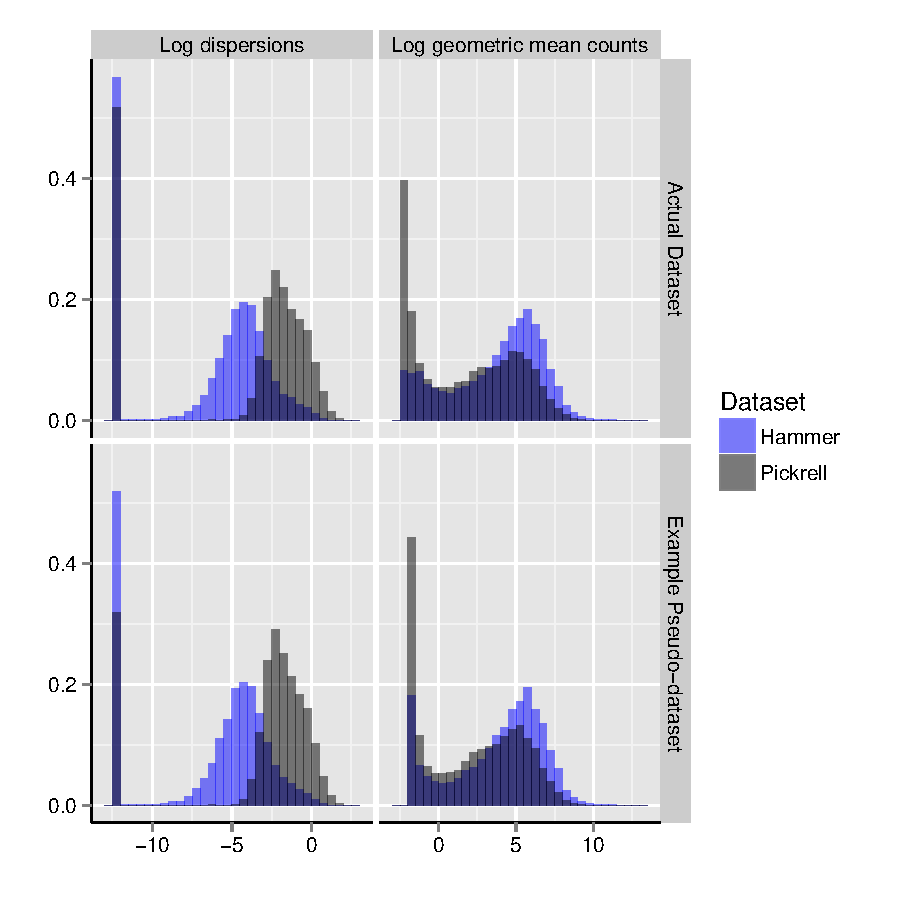
\includegraphics{../fig/hists_slides}
\end{frame}

\begin{frame}
\frametitle{The Underlying Real Datasets}
\setkeys{Gin}{height=0.9\textheight}
\setkeys{Gin}{width=1\textwidth}
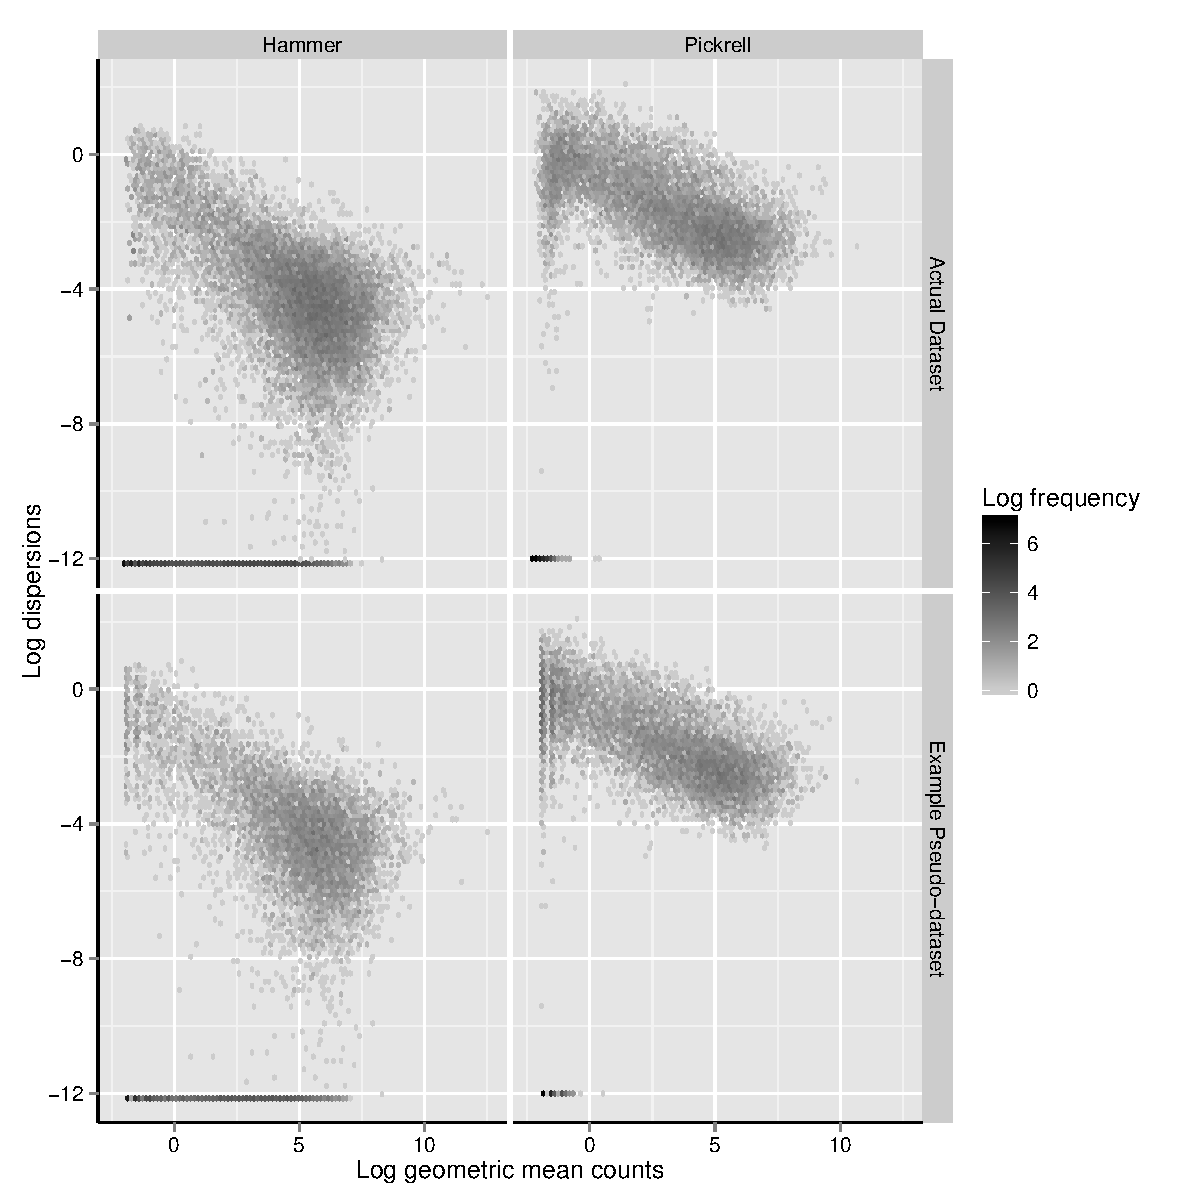
\includegraphics{../fig/meandisp_scatter_slides}
\end{frame}







\begin{frame}
\frametitle{Simulation Settings}
\begin{tabular}{llll}
Setting & Dataset & Group 1 Libraries & Group 2 Libraries \\ \hline
I & Pickrell & 3 & 3 \\
II & Pickrell & 3 & 15 \\
III & Pickrell & 9 & 9 \\
IV & Hammer & 3 & 3 \\
V & Hammer & 3 & 16 \\
VI & Hammer & 9 & 9 \\
\end{tabular} 
\end{frame}

\section{Results}
\begin{frame}
\frametitle{Mean Squared Error}
Mean squared error of adjusted dispersions:

\begin{align*}
\text{MSE} = \frac{1}{10000} \sum_{h = 1}^{10000} \left [\frac{\wh{\phi}_h}{1 + \wh{\phi}_h} - \frac{\phi_h}{1 + \phi_h} \right ] ^2
\end{align*}
\end{frame}


\setkeys{Gin}{height=.8\textheight}

\begin{frame}
\frametitle{\small MSEs of the pseudo-datasets of simulation settings I, II, and III}
\begin{center}

\setkeys{Gin}{width=0.9\textwidth}
\begin{center}
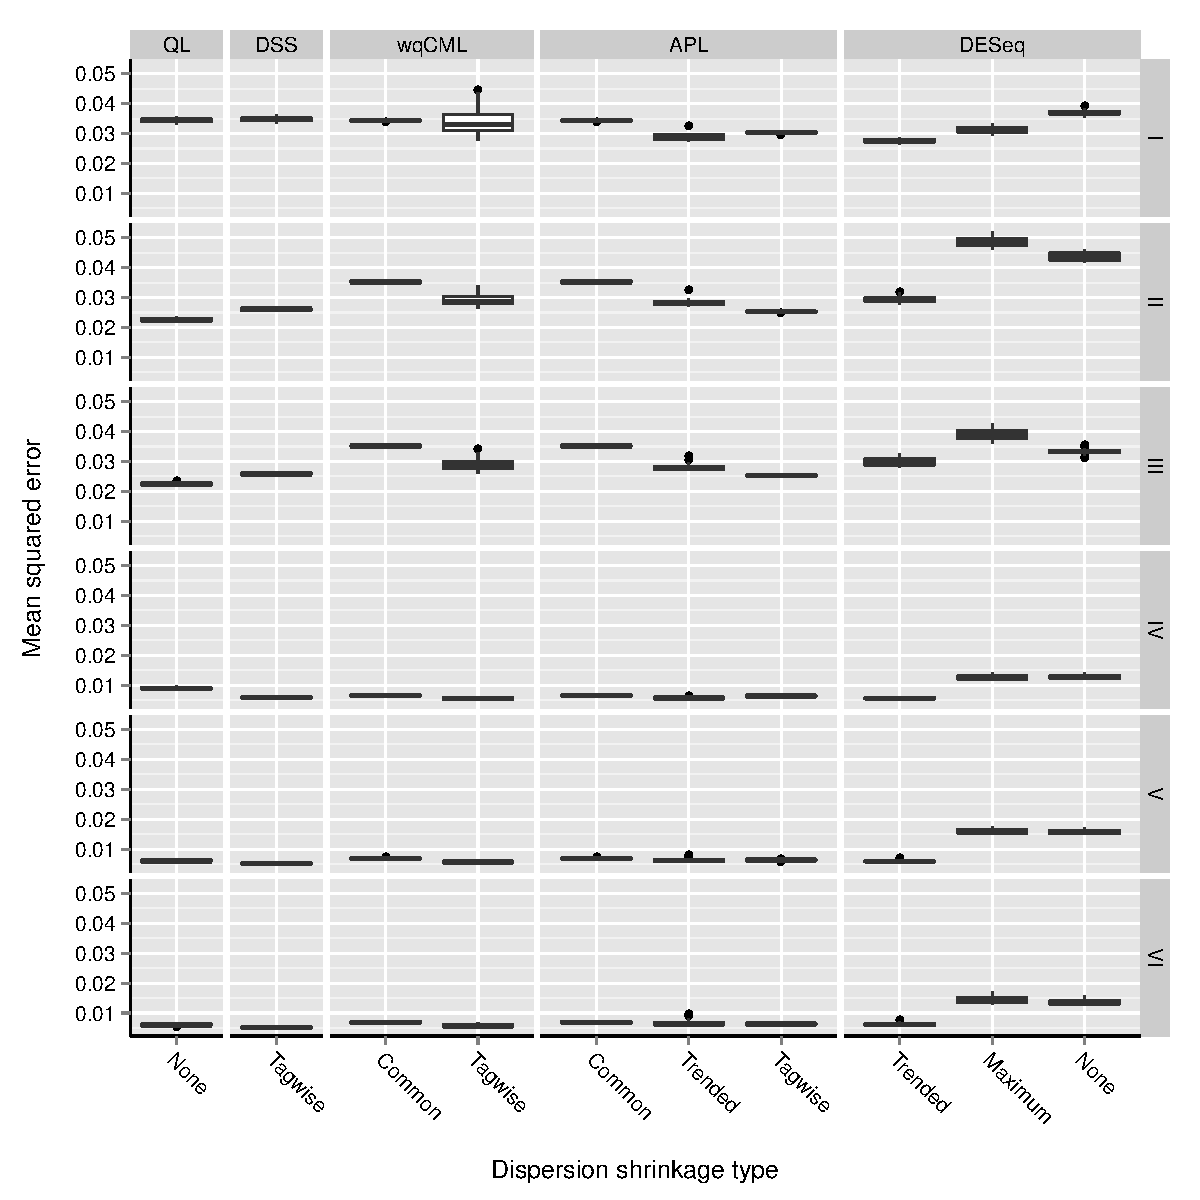
\includegraphics{../fig/mse_slides}
\end{center}
\end{center}
\end{frame}

\begin{frame}
\frametitle{Estimated vs. True Dispersions: Simulation Setting I}
\begin{center}
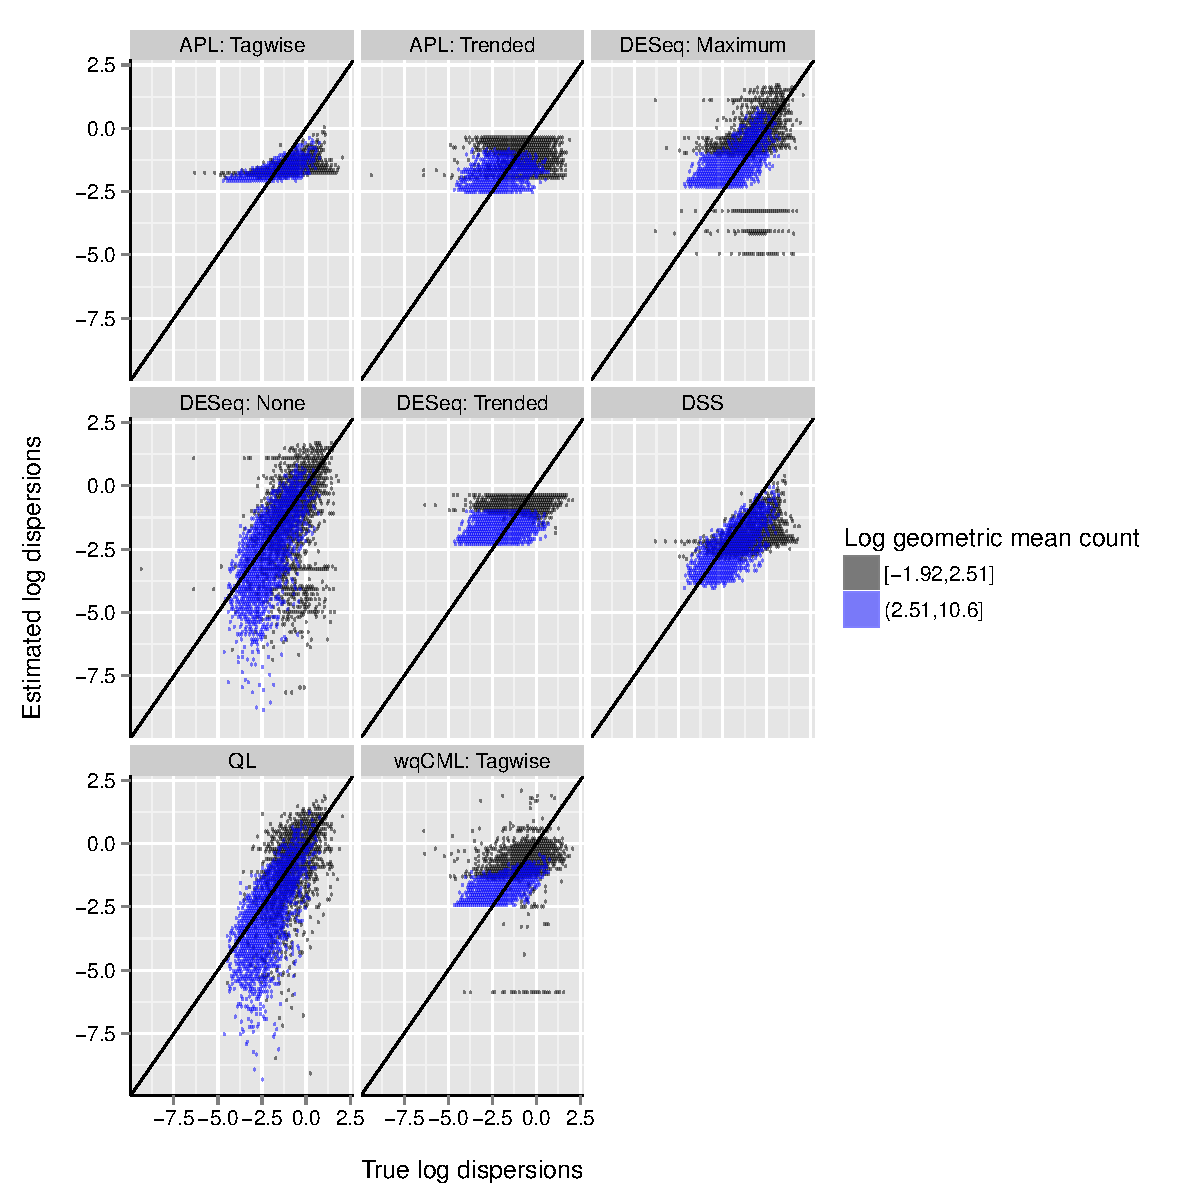
\includegraphics{../fig/phi_vs_phi_I_slides} 
\end{center}
\end{frame}

\begin{frame}
\frametitle{Estimated vs. True Dispersions: Simulation Setting II}
\begin{center}
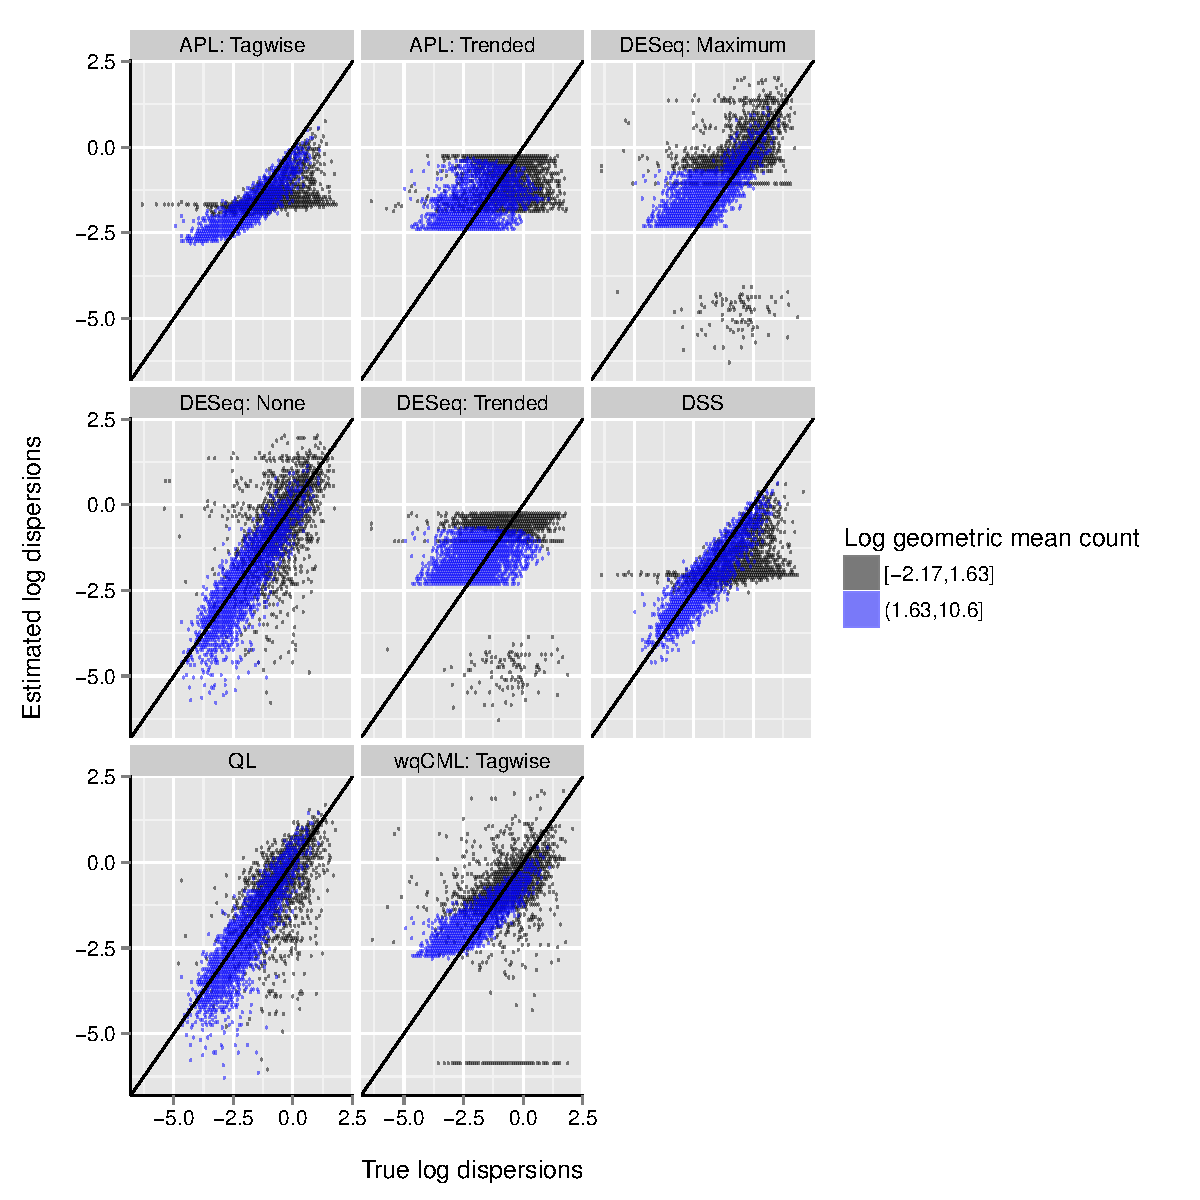
\includegraphics{../fig/phi_vs_phi_II_slides} 
\end{center}
\end{frame}

\begin{frame}
\frametitle{Estimated vs. True Dispersions: Simulation Setting III}
\begin{center}
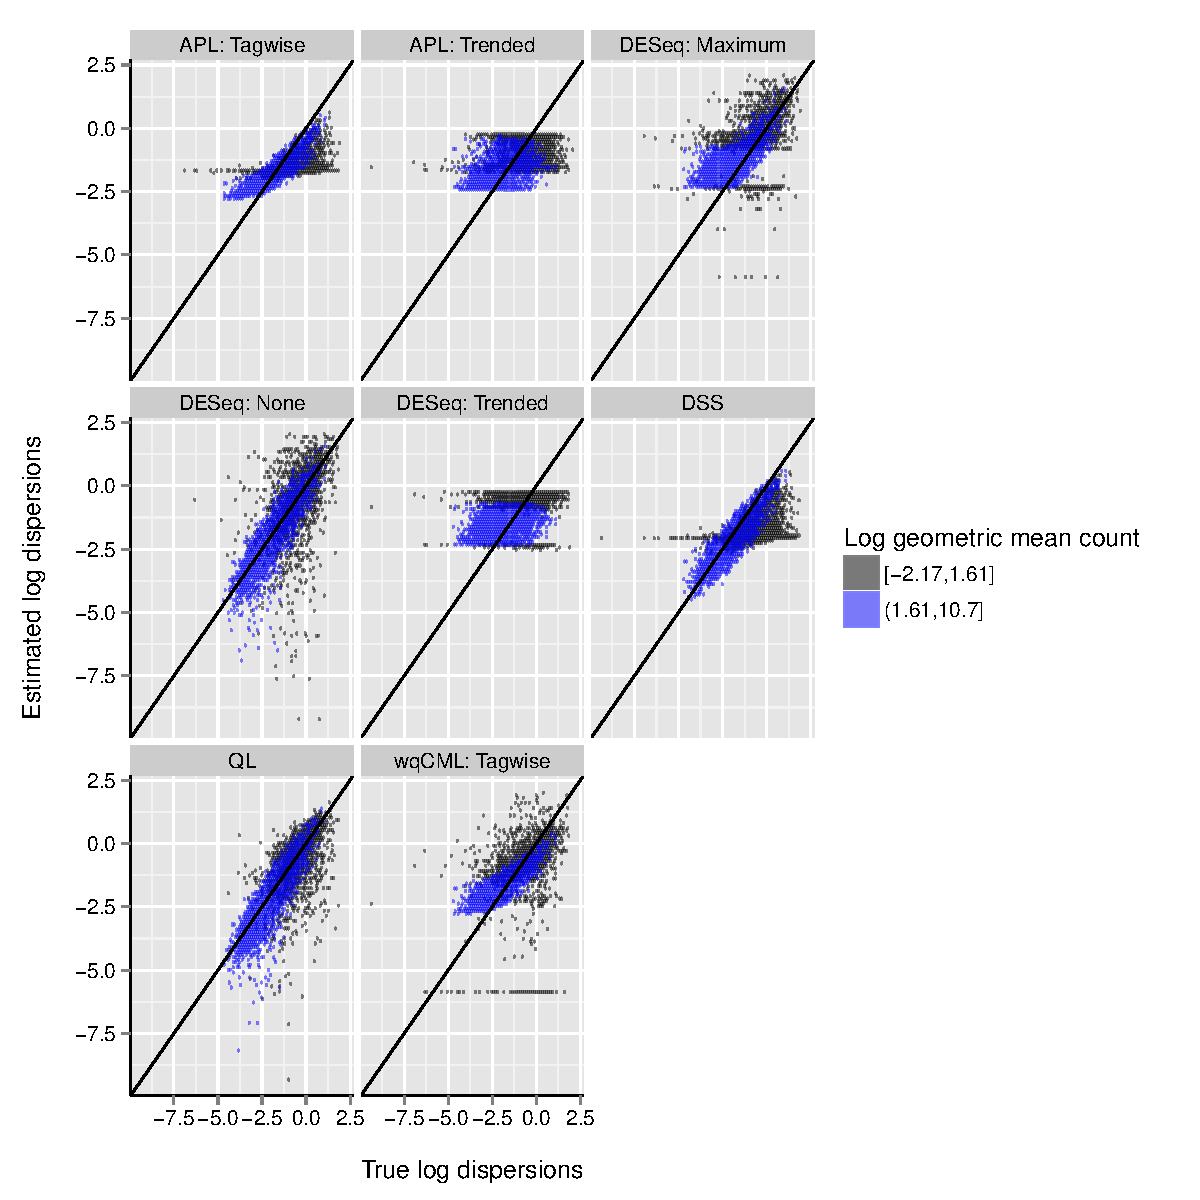
\includegraphics{../fig/phi_vs_phi_III_slides} 
\end{center}
\end{frame}

\begin{frame}
\frametitle{Estimated vs. True Dispersions: Simulation Setting IV}
\begin{center}
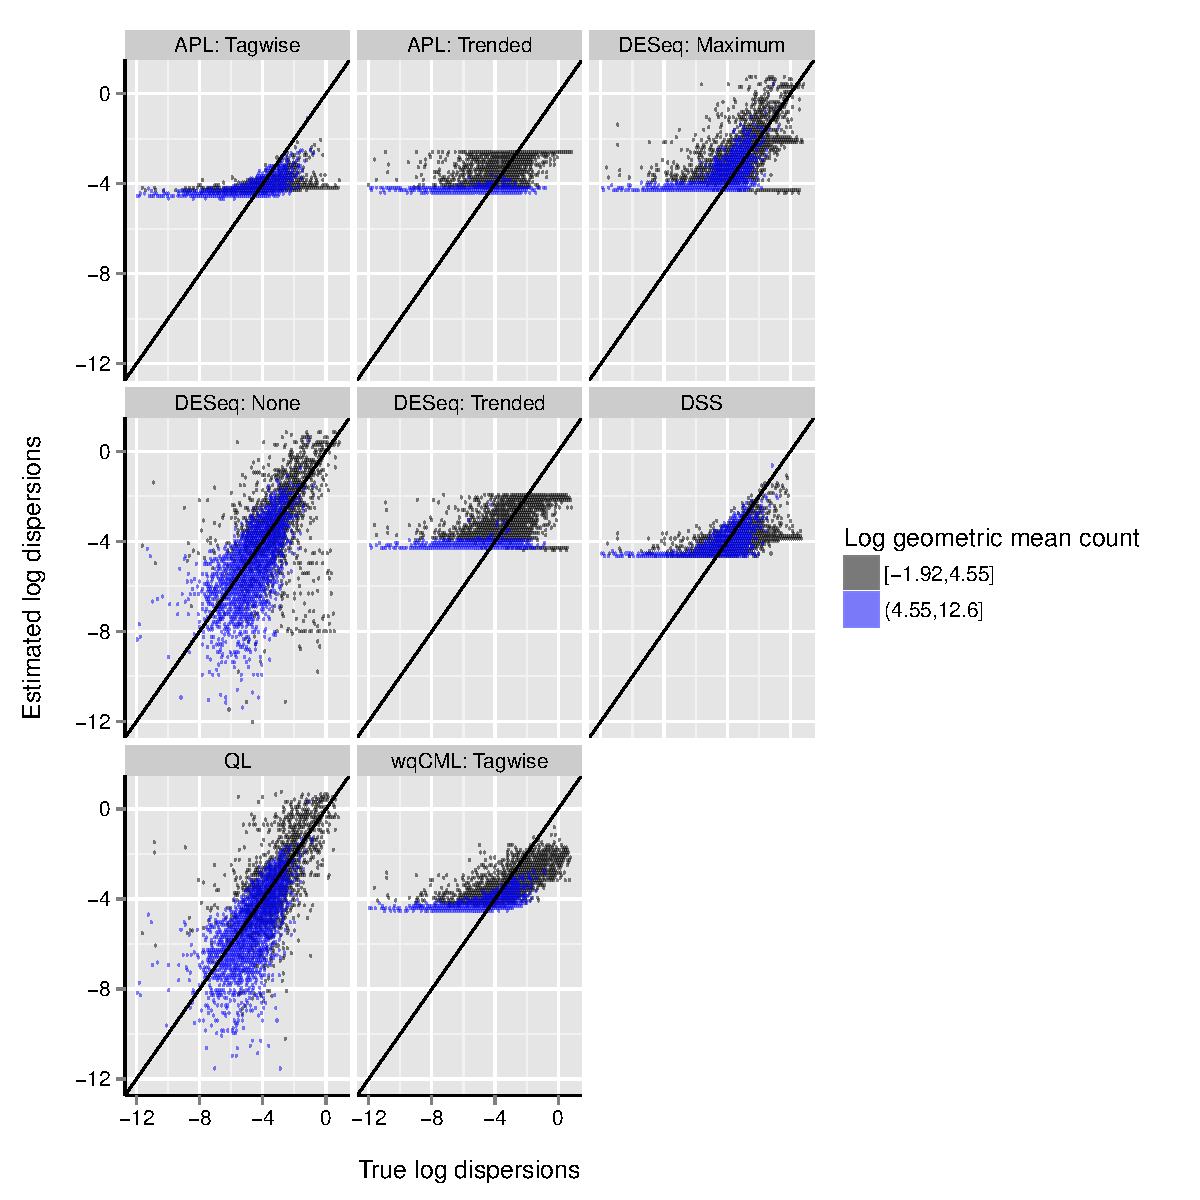
\includegraphics{../fig/phi_vs_phi_IV_slides} 
\end{center}
\end{frame}

\begin{frame}
\frametitle{Estimated vs. True Dispersions: Simulation Setting V}
\begin{center}
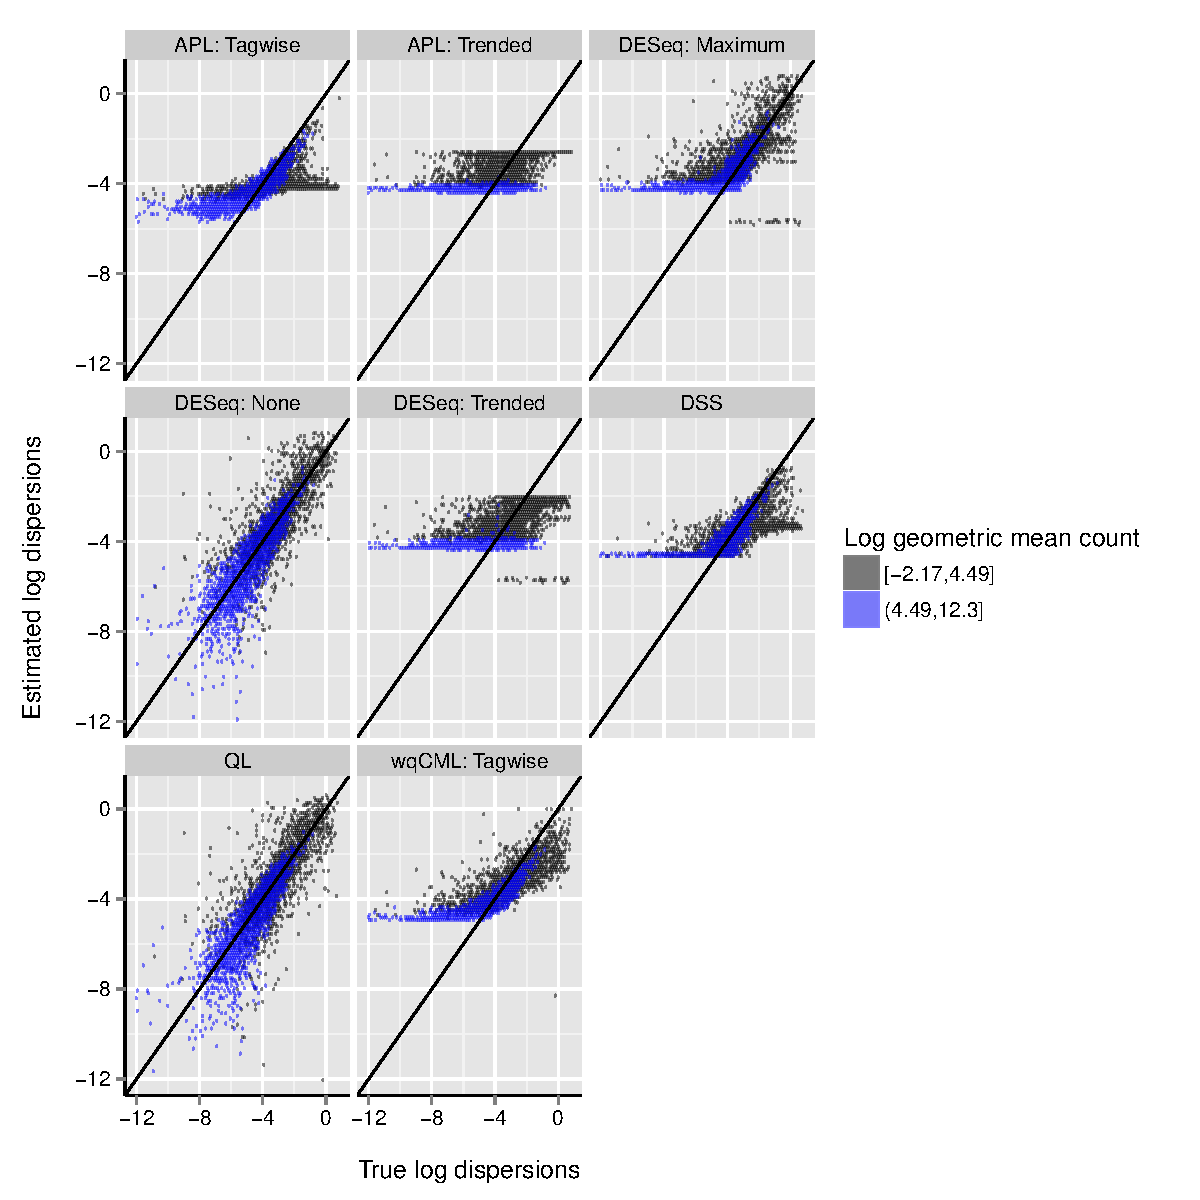
\includegraphics{../fig/phi_vs_phi_V_slides} 
\end{center}
\end{frame}

\begin{frame}
\frametitle{Estimated vs. True Dispersions: Simulation Setting VI}
\begin{center}
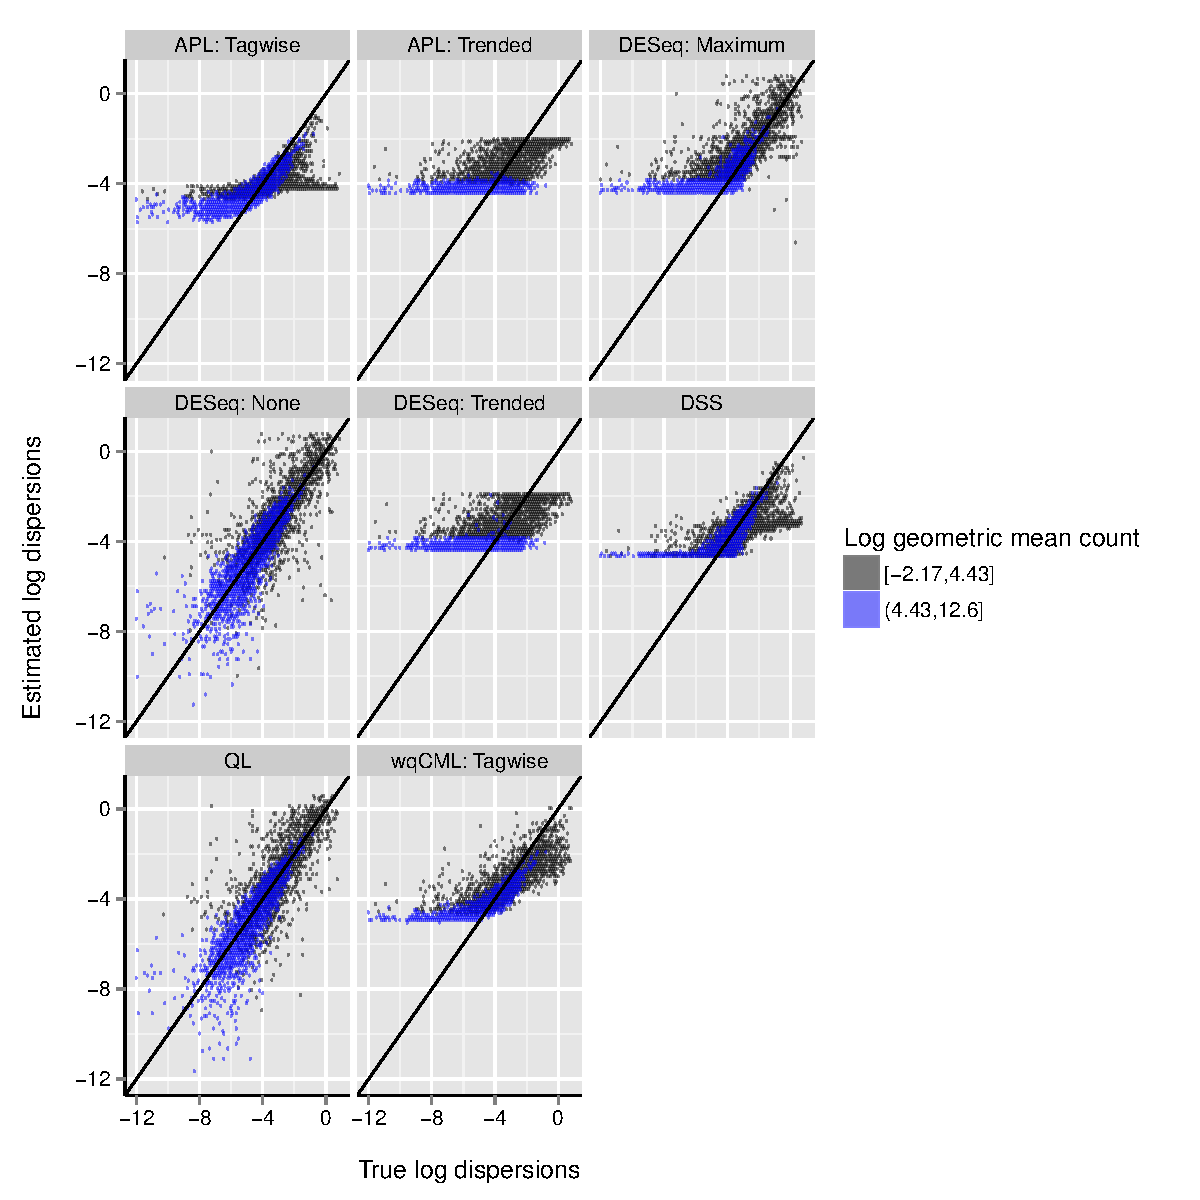
\includegraphics{../fig/phi_vs_phi_VI_slides} 
\end{center}
\end{frame}





\begin{frame}
\frametitle{\small Effect of dispersion estimation method on DE test performance}
\scriptsize
\begin{itemize}
\pause \item Receiver operating characteristic (ROC) curve: graph of the true positive rate (TPR) of DE gene detection on the false positive rate (FPR) for several values of FPR from 0 to 1.
\begin{itemize}
\pause \item TPR: ratio of correctly identified DE genes to all the actually DE genes.
\pause \item FPR ratio of genes incorrectly identified as DE to all the actually EE genes.
\end{itemize}
\pause \item The areas under the ROC curves (AUC) for FPR $< 0.2$ were plotted for each combination of simulation, dispersion, and test settings.
\end{itemize}

\begin{center}
\setkeys{Gin}{height=.475\textheight}
\setkeys{Gin}{width=.475\textwidth}
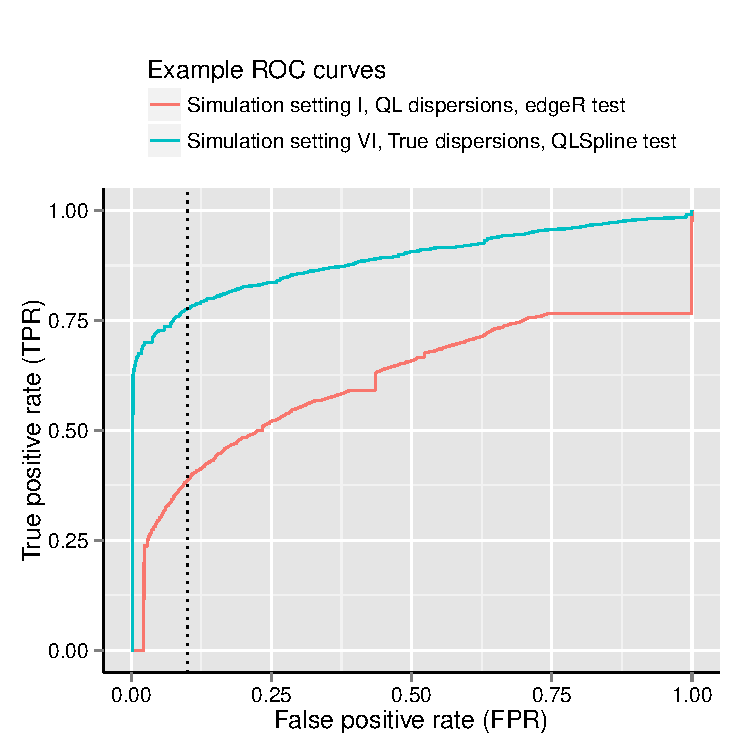
\includegraphics{../fig/roc_slides}
\end{center}

\end{frame}

\setkeys{Gin}{height=.9\textheight}
\setkeys{Gin}{width=0.9\textwidth}

\begin{frame}
\frametitle{\small AUCs: Simulation Setting I}
\begin{center}
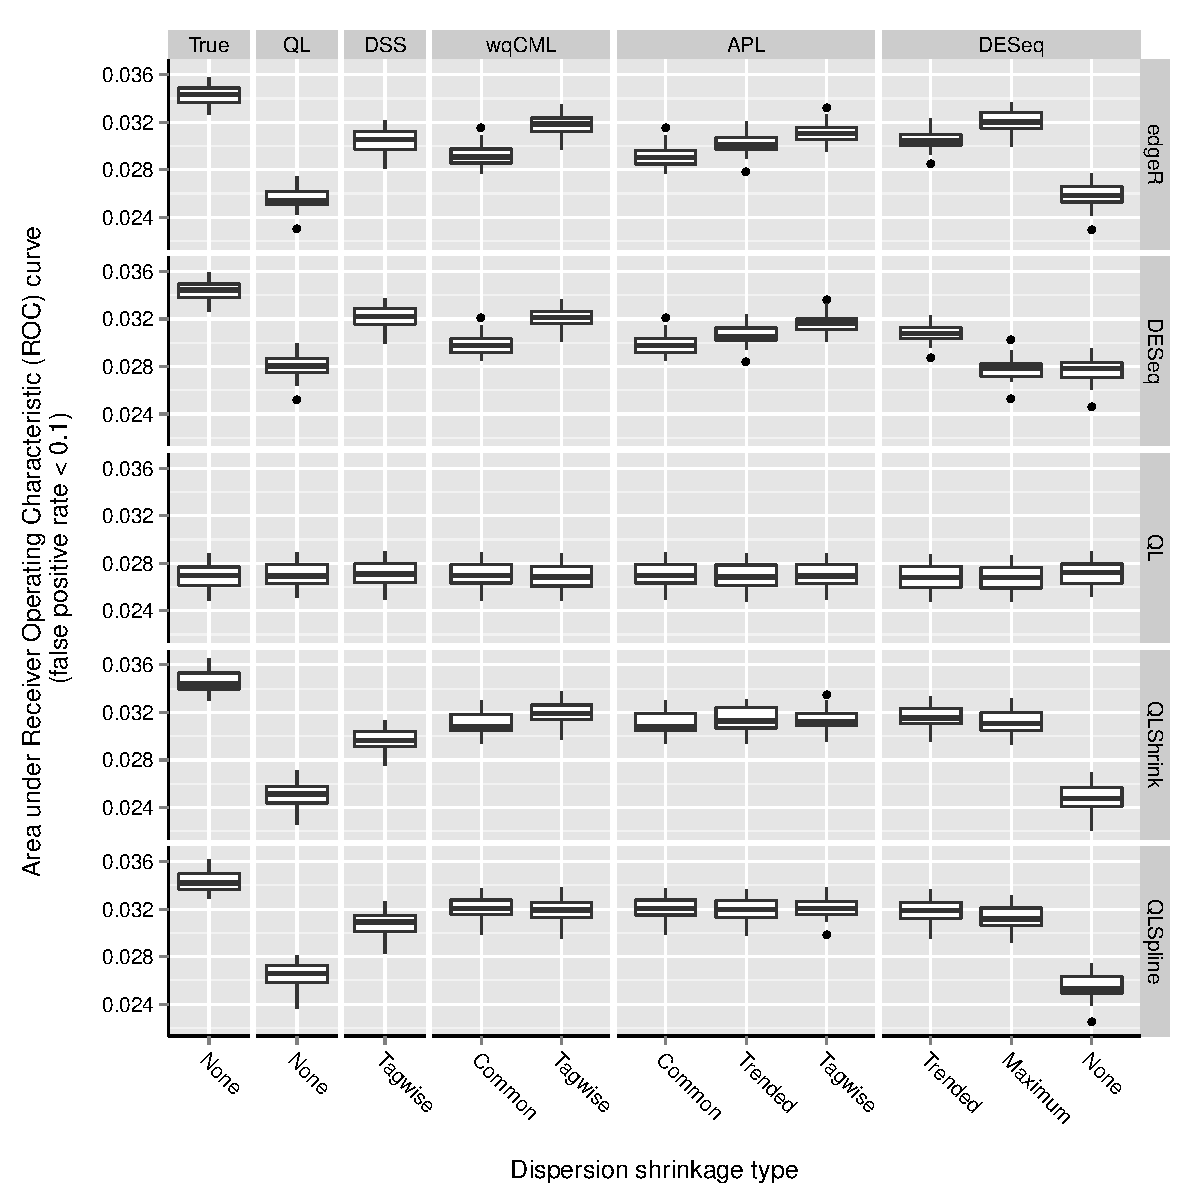
\includegraphics{../fig/auc1_slides}
\end{center}
\end{frame}

\begin{frame}
\frametitle{\small AUCs: Simulation Setting II}
\begin{center}
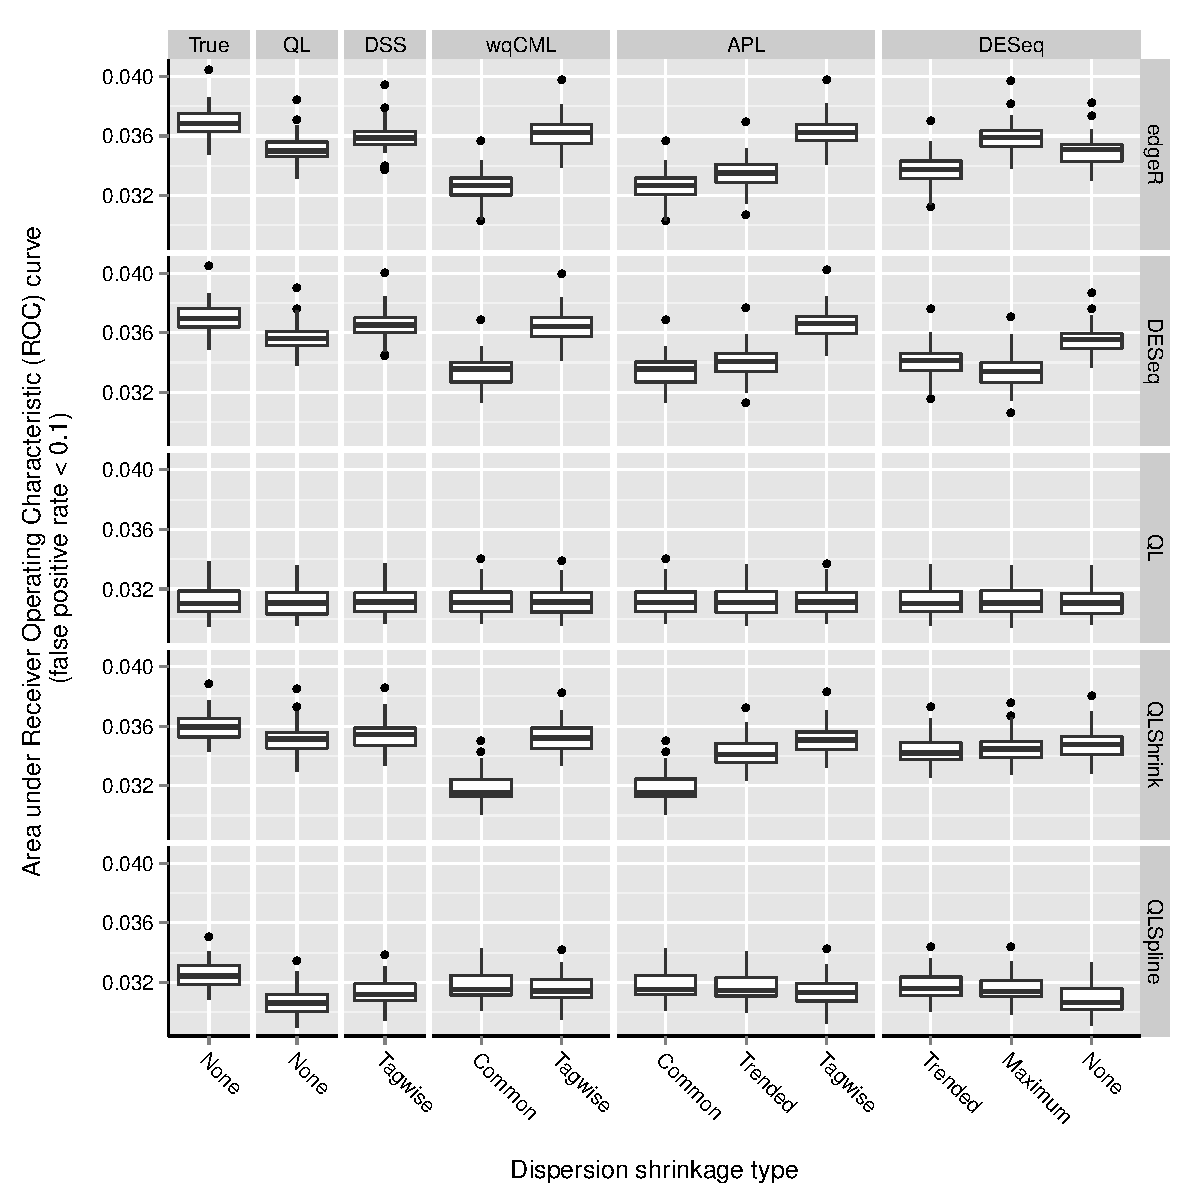
\includegraphics{../fig/auc2_slides}
\end{center}
\end{frame}

\begin{frame}
\frametitle{\small AUCs: Simulation Setting III}
\begin{center}
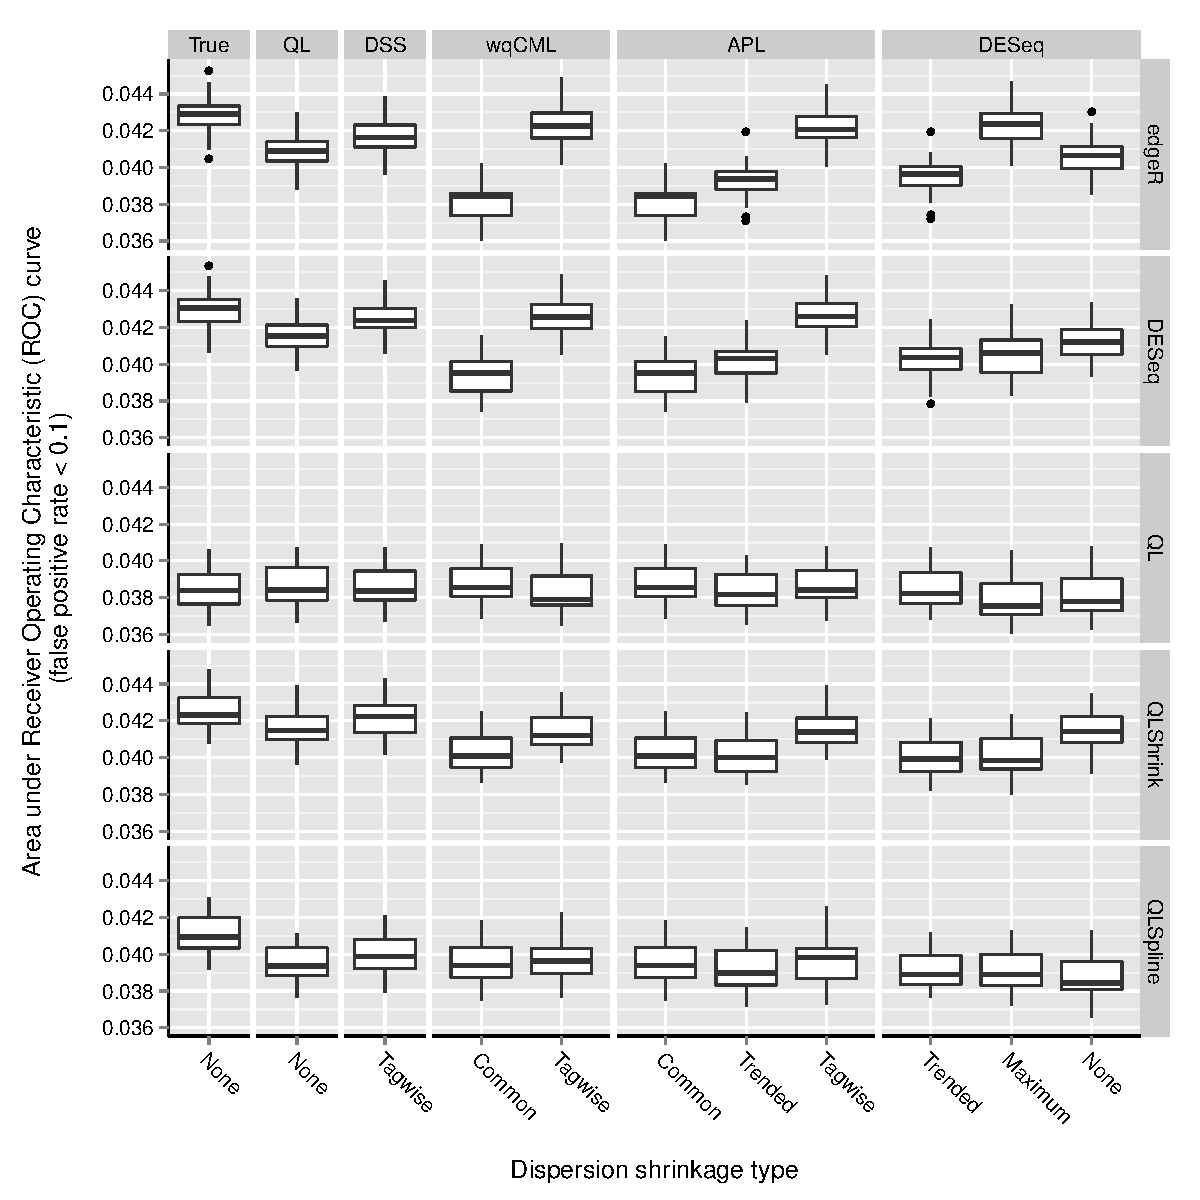
\includegraphics{../fig/auc3_slides}
\end{center}
\end{frame}

\begin{frame}
\frametitle{\small AUCs: Simulation Setting IV}
\begin{center}
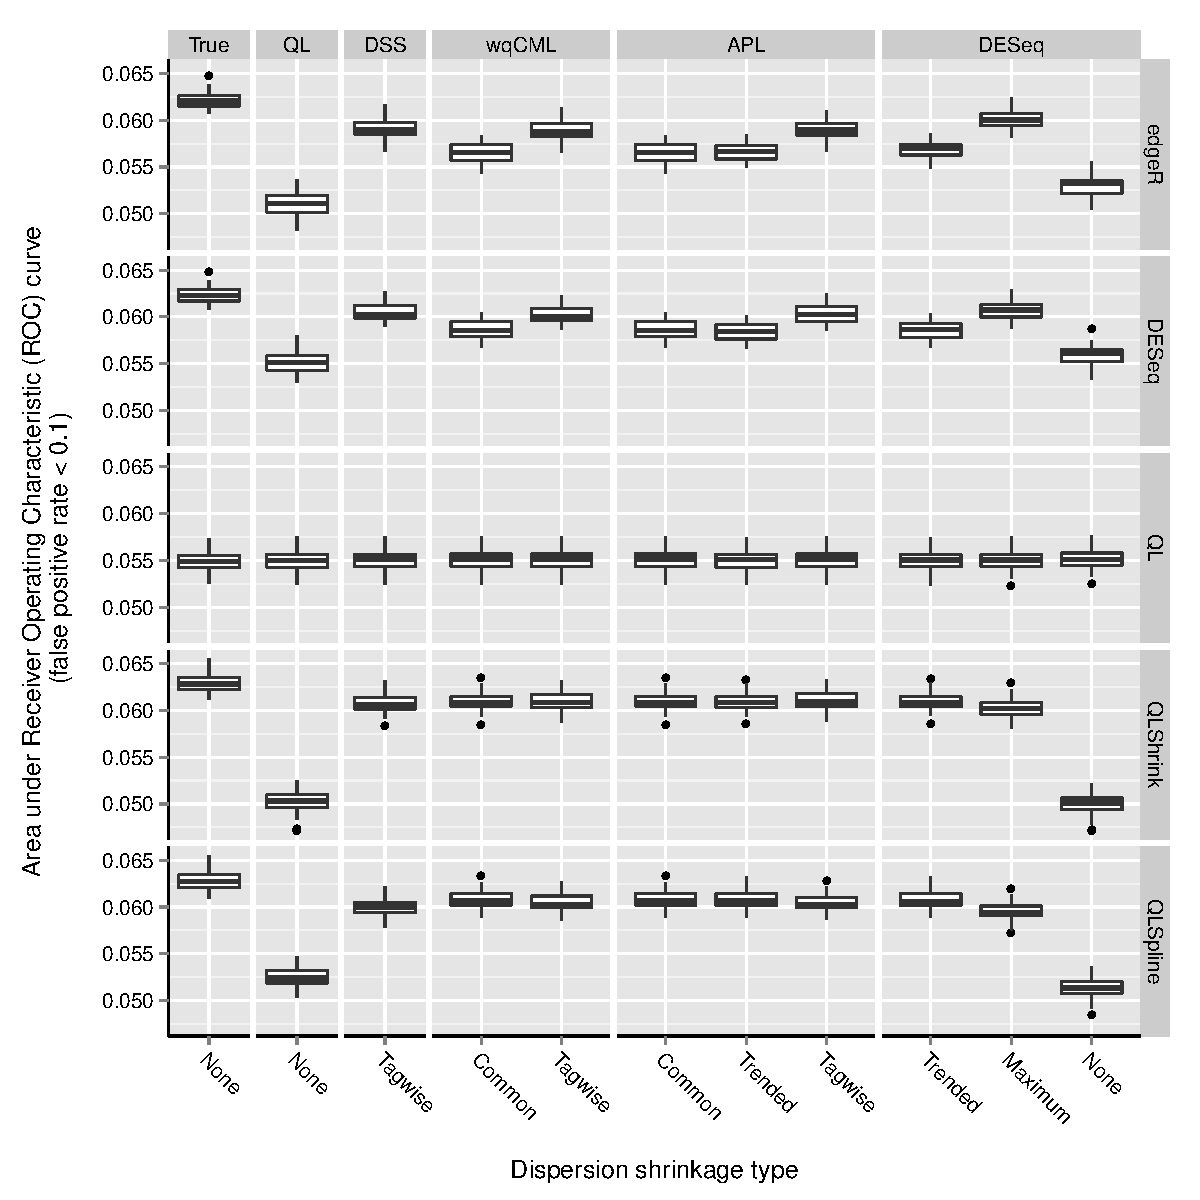
\includegraphics{../fig/auc4_slides}
\end{center}
\end{frame}

\begin{frame}
\frametitle{\small AUCs: Simulation Setting V}
\begin{center}
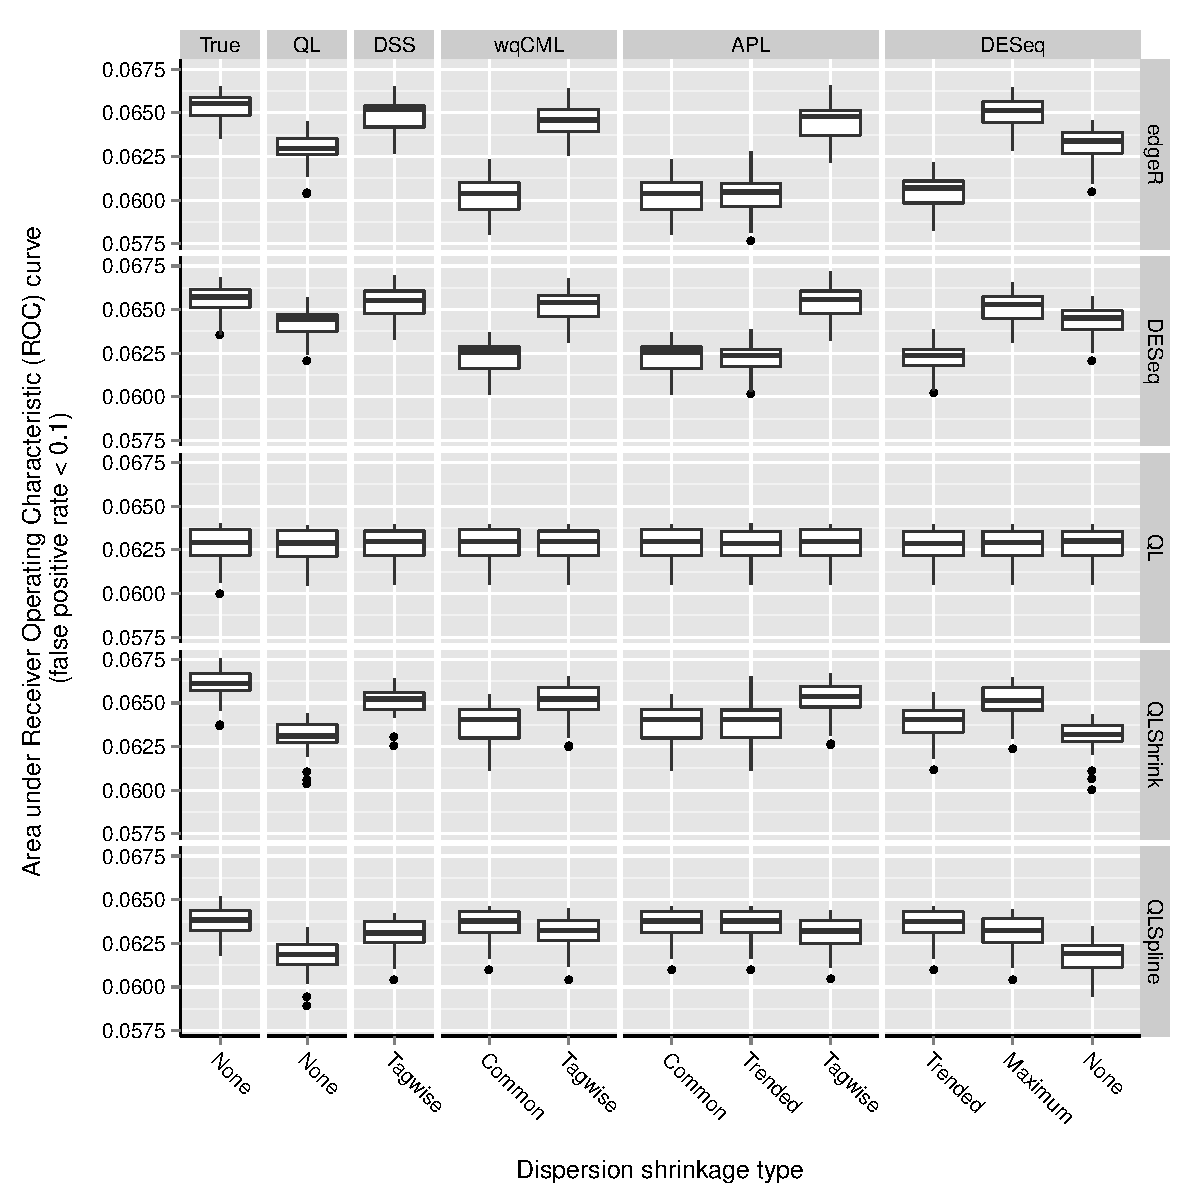
\includegraphics{../fig/auc5_slides}
\end{center}
\end{frame}

\begin{frame}
\frametitle{\small AUCs: Simulation Setting VI}
\begin{center}
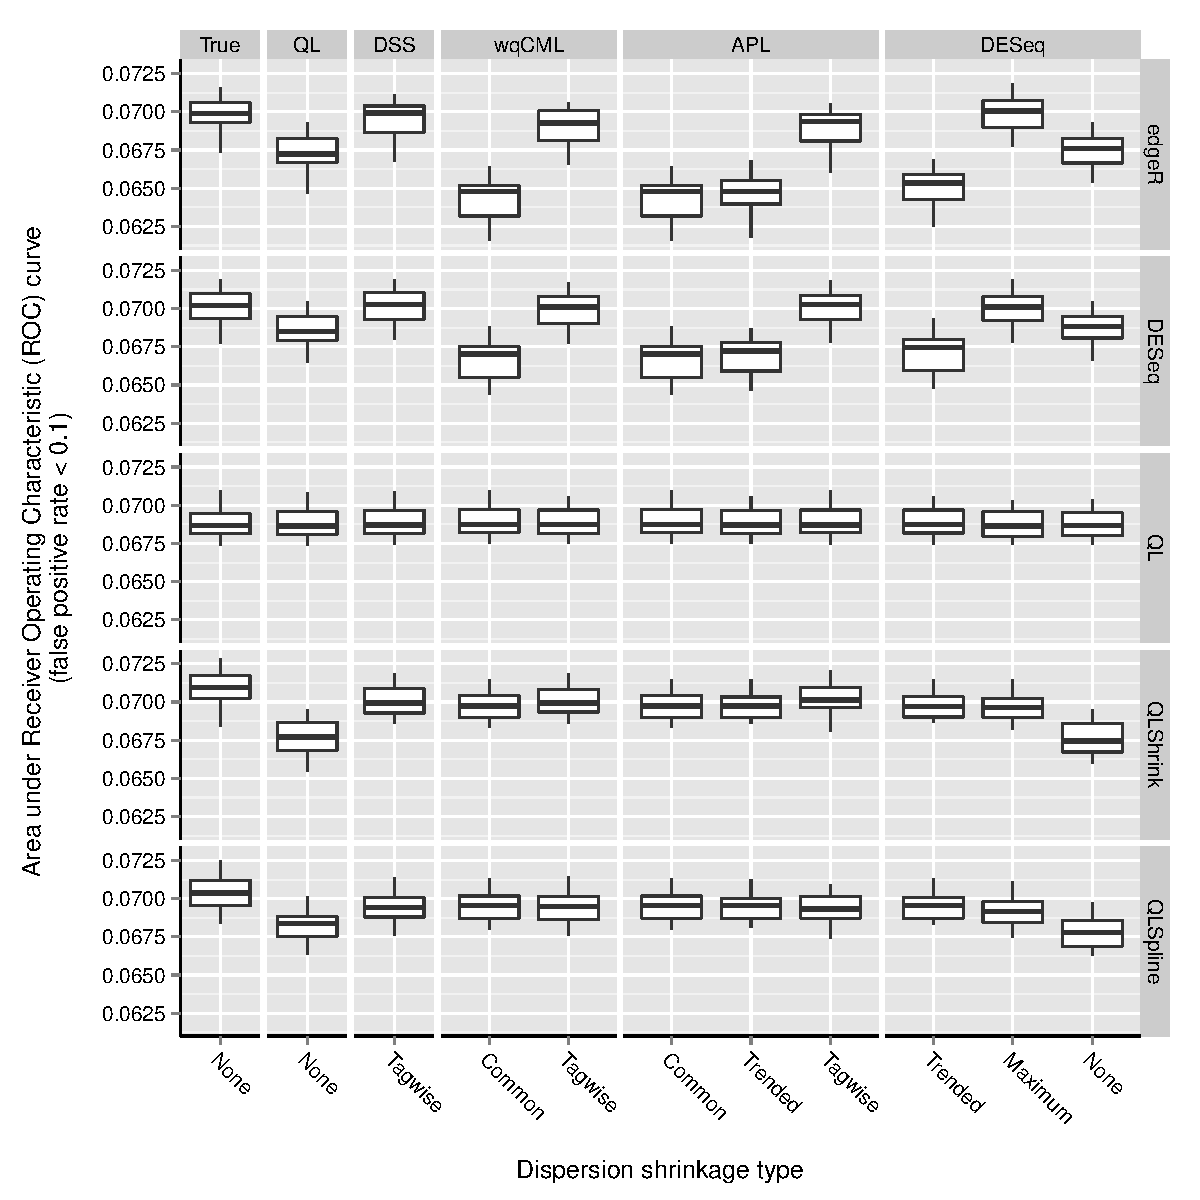
\includegraphics{../fig/auc6_slides}
\end{center}
\end{frame}


\section{Conclusions}

\begin{frame}
\frametitle{Conclusions}

\begin{itemize}
\item Overall, the mean squared error-best methods are the ones that set the dispersions to a common trend (heavy shrinkage to a trend).
\pause \item The dispersions estimated independently for each gene (no shrinkage) have the strongest linear relationships with the true dispersions.
\pause \item The ones that maximize the performance of tests for differential expression are the ones that use a moderate degree of dispersion shrinkage, regardless of whether this shrinkage is toward a common value, trend, or prior distribution.
\end{itemize}
\end{frame}

\begin{frame}
\frametitle{Exceptions}

\begin{itemize}
\item Tagwise APL method is one of the mean squared error-best methods even though it is not one of the trended methods.
\pause \item The DSS and wqCML dispersions have strong linear relationships with the true dispersions for many of the Pickrell simulation settings despite the fact that these methods use some form of dispersion shrinkage. 
\end{itemize}
\end{frame}


\begin{frame}
\frametitle{Acknowledgements}
We would like to thank Dr. Dan Nettleton, Dr. Dianne Cook, Dr. Long Qu, Emily King, Yet Tien Nguyen, and Fangfang Liu of Iowa State University for their useful feedback. We would also like to thank Dr. Gordon Smyth of the Walter and Eliza Hall Institute in Australia for answering our questions.
\end{frame}

\begin{frame}[allowframebreaks]
\frametitle{Sources} \scriptsize
\begin{enumerate}[1. ]
\item S. Anders and W. Huber. Differential expression analysis for sequence count data. \emph{Genome Biology}, 11(10), October 2010.
\item A. C. Cameron and P. K. Travedi. \emph{Regression Analysis of Count Data}. Cambridge University Press, 1998.
\item Robert C Gentleman, Vincent J. Carey, Douglas M. Bates, and others. Bioconductor: Open software development for computational biology and bioinformatics. \emph{Genome Biology}, 5:R80, 2004. \url{http://genomebiology.com/2004/5/10/R80}.
\item P. Hammer, M. S. Banck, R. Amberg, et al. mrna-seq with agnostic splice site discovery for nervous system transcriptomics tested in chronic pain. \emph{Genome Research}, 20(6):847�60, June 2010.
\item S. Lund. Package �QuasiSeq�. \url{http://cran.r-project.org/web/packages/QuasiSeq/QuasiSeq.pdf}, June 2012.
\item S. P. Lund, D. Nettleton, D. J. McCarthy, and G. K. Smyth. Detecting differential expression in RNA-sequence data using quasi-likelihood with shrunken dispersion estimates. \emph{Statistical Applications in Genetics and Molecular Biology}, 11(5), October 2012.
\item D. J. McCarthy, Y. Chen, and G. K. Smyth. Differential expression analysis of multifactor RNA-seq experiments with respect to biological variation. \emph{Nucleic Acids Research}, 40:4288�97, 2012.
\item P. McCullagh. Quasi-likelihood functions. \emph{Annals of Statistics}, 11:59�67, 1983.
\item A. Oshlack, M. D. Robinson, and M. D. Young. From RNA-seq reads to differential expression results. \emph{Genome Biology}, 11(220), 2010.
\item J. K. Pickrell, J. C. Marioni, A. A. Pai, et al. Understanding mechanisms underlying human gene expression variation with RNA sequencing. \emph{Nature}, 464(7289):768�72, April 2010.
\item R Core Team. R: A Language and Environment for Statistical Computing. R Foundation for Statistical Computing, Vienna, Austria, 2012. \url{http://www.R-project.org. ISBN 3-900051-07-0}.
\item M. D. Robinson and A. Oshlack. A scaling normalization method for differential expression analysis of RNA-seq data. \emph{Genome Biology}, 11(3), 2010.
\item M. D. Robinson and G. K. Smyth. Moderated statistical tests for assessing differences in tag abundance. \emph{Bioinformatics}, 23(21):2881�2887, 2007.
\item M. D Robinson and G. K. Smyth. Small-sample estimation of negative binomial dispersion, with applications to sage data. \emph{Biostatistics}, 9(2): 321�332, 2008.
\item M. D. Robinson, D. J. McCarthy, and G. K. Smyth. edgeR: a Bioconductor package for differential expression analysis of digital gene expression data. \emph{Bioinformatics}, 26(1):139�140, October 2009.
\item M. D. Robinson, D. J. McCarthy, Y. Chen, and G. K. Smyth. Package �edgeR�. \url{http://www.bioconductor.org/packages/2.10/bioc/ manuals/edgeR/man/edgeR.pdf}, September 2012.
\item Y. Si. Package �AMAP.Seq�. \url{http://cran.r-project.org/web/packages/AMAP.Seq/AMAP.Seq.pdf}, June 2012.
\item Y. Si and P. Liu. An optimal test with maximum average power while controlling FDR with application to RNA-seq data. Accepted, 2012.
\item L. Wang, P. Li, and T. P. Brutnell. Exploring plant transcriptomes using ultra high-throughput sequencing. \emph{Briefings in Functional Genomics}, 9 (2):118�128, 2010. doi: 10.1093/bfgp/elp057. \url{http://bfg.oxfordjournals.org/content/9/2/118.abstract}.
\item H. Wu, C. Wang, and Z. Wu. A new shrinkage estimator for dispersion improves differential expression detection in RNA-seq data. \emph{Biostatistics}, 1 (1):1�24, 2012.
\end{enumerate}
\end{frame}





















































%%%%%%%%%%%%%%%
%%%%%%%%%%%%%%%
%%%%%%%%%%%%%%%
%%%%%%%%%%%%%%%
%%%%%%%%%%%%%%%
%%%%%%%%%%%%%%%
%%%%%%%%%%%%%%%
%%%%%%%%%%%%%%%
%%%%%%%%%%%%%%%
%%%%%%%%%%%%%%%

\appendix

\section{Appendix: Dispersion Estimation Methods in Detail}

\subsubsection{QL}


\begin{frame}
\frametitle{\small The quasi-likelihood (QL) method (Robinson and Smyth, 2007)}
\small
\begin{itemize}
\pause \item Implementation: package {\tt AMAP.Seq} (Si and Liu, 2012)
\pause \item Algorithm: 
\begin{enumerate}[1. ]
\pause \item Set $\wh{\phi}_g$, the estimate of $\phi_g$, to some initial value.
\pause \item Calculate the MLE, $\wh{\mu}_{g, i}$, of each ``true" unnormalized count mean, $\mu_{g, i}$, by maximizing the negative binomial log likelihood given $\phi_g = \wh{\phi}_g$ and count $y_{g, i}$.
\pause \item Update $\wh{\phi}_g$ to be the quasi-likelihood tagwise dispersion estimate given $\mu_{g, i} = \wh{\mu}_{g, i}$ by solving for $\wh{\phi_g}$:

\pause \begin{align*}
2 \sum_{i = 1}^n & \left \{ y_{g, i} \log \left [ \frac{y_{g, i}}{\wh{\mu}_{g, i}} \right ] - (y_{g, i} + \wh{\phi}_g \nv) \log \left [ \frac{y_{g, i} + \wh{\phi}_g \nv}{\wh{\mu}_{g, i} + \wh{\phi}_g \nv} \right ] \right \} 
\\ &= n - 1
\end{align*}
\pause \item Iterate steps 2-4 a pre-determined number of times, each time using the most current value of $\wh{\phi}_g$.

\end{enumerate}
\end{itemize}

\end{frame}

 
\subsubsection{DSS}


\begin{frame}
\frametitle{\small The dispersion shrinkage for sequencing (DSS) method (Wu, Wang, and Wu, 2012)}
\small

\begin{itemize}
\pause \item Idea: shrink $\wh{\phi}_g$ towards a common \emph{prior} instead of a common value.
\pause \item Model:
\begin{align*}
\uncover<4->{Y_{g, i} \mid \theta_{g, i}} & \uncover<4->{\sim \text{Poisson}(\theta_{g, i} s_i)} \\
\uncover<5->{\theta_{g, i} \mid \phi_g} & \uncover<5->{\sim \text{Gamma}(\nu_{g, k(i)}, \phi_g)} \\
\uncover<6->{\phi_g} & \uncover<6->{\sim \text{log-normal}(m_0, \tau^2)}
\end{align*}
\pause \pause \pause
\pause \item The marginal distribution of the $Y_{g, i}$'s is NB($\mu_{g, i}, \phi_g$), where $\mu_{g, i} = s_i \nu_{g, k(i)}$ as before.
\pause \item Implementation: package {\tt DSS}
\end{itemize}
\end{frame}

\begin{frame}
\frametitle{\small Estimating $\phi_g$}

\begin{itemize}
\pause \item Estimate hyperparameters $m_0$ and $\tau^2$ using the method of moments estimates of $\phi_g$.
\pause \item $\wh{\nu}_{g, k(i)} = \frac{\sum_{j:k(j) = k(i)} Y_{g, j} / s_j}{n_{k(i)}}$,  where $n_{k(i)}$ is the number of libraries in the same treatment group as replicate $i$.
\pause \item Set $\wh{\mu}_{g, i} = s_i \wh{\nu}_{g, k(i)}$ as before.
\pause \item Take $\wh{\phi}_g$ to be the mode of the posterior density, $f(\phi_g \mid Y_{g, i}, \mu_{g, i}, i = 1, \ldots, n)$, given by:

\scriptsize
\pause \begin{align*}
\log[f(\phi_g & \mid Y_{g, i}, \mu_{g, i}, i = 1, \ldots, n)] \\
&\propto \sum_i \psi(\phi_g \nv + Y_{g, i}) \\
&- n \psi(\phi_g \nv) - \phi_g \nv \sum_i \log(1 + \mu_{g, i} \phi_g) \\
&+ \sum_i Y_{g, i} [\log(\mu_{g, i} \phi_g) - \log(1 + \mu_{g, i} \phi_g)] \\
&- \frac{[\log(\phi_g) - m_0]^2}{2 \tau^2} - \log(\phi_g) - \log(\tau)      
\end{align*}

\end{itemize}
\end{frame}



\subsubsection{wqCML}

\begin{frame}
\frametitle{\small The weighted quantile-adjusted conditional maximum likelihood (wqCML) method (Robinson \& Smyth, 2007)}
\small
\begin{itemize}
\pause \item Implementation:
\begin{itemize}
\pause \item Package {\tt edgeR}.
\pause \item Use the {\tt estimateTagwiseDisp()} function.
\pause \item Set $\alpha$ with the {\tt prior.n} argument.
\end{itemize}

\pause \item Maximize the weighted likelihood:

\pause \begin{align*}
\text{WL}(\phi_g) = l_g(\phi_g) + \alpha l_C(\phi_g)
\end{align*}

\begin{itemize}
\pause \item  $l_C$: the ``common" log likelihood, the negative binomial log likelihood under the restriction that all genes share the same dispersion value.
\pause \item $l_g$: the log likelihood given by quantile-adjusted conditional maximum likelihood (qCML).
\pause \item $\alpha$: tuning parameter, typically calculated via empirical Bayes.
\end{itemize}
\end{itemize}
\end{frame}




\begin{frame}
\frametitle{\small Conditional maximum likelihood (CML): the basis for qCML}
\small

\begin{itemize}
\pause \item Assume:
\begin{itemize}
\pause \item Each library has $m$ total reads.
\pause \item $Y_{g, 1}, \ldots, Y_{g, n}$ are mutually independent.
\end{itemize}

\pause \item Then:
\begin{itemize}
\pause \item $Y_{g, i} \sim $ NB($m \nu_{g, k(i)}$, $\phi_g$).
\pause \item $Z_g = \sum_{i = 1}^n Y_{g, i} \sim \text{NB}(nm\nu_{g, k(i)}, \phi_g)$
\end{itemize}


\pause \item CML selects the $\wh{\phi}_g$ that maximizes the log likelihood of $Y_g = (Y_{g, 1}, \ldots, Y_{g, n})$ conditioned on $Z_g$ in terms of $\phi_g$:
\pause \begin{align*}
l_{Y_{g} \mid Z_g = z}(\phi_g) &= \left [ \sum_{i = 1}^n \log \Gamma(y_{g, i} + \phi_g \nv) \right ] + \log \Gamma(n \phi_g \nv) \\
&- \log \Gamma(z + n \phi_g \nv) - \log \Gamma(\phi_g \nv)
\end{align*}
\end{itemize}
\end{frame}


\begin{frame}
\frametitle{\small Quantile-adjusted CML (qCML)} \scriptsize
\pause Now, assume $y_{g, i}$ is drawn from $Y_{g, i} \sim$ NB($m_i \nu_{g, k(i)}, \phi_g)$, where the library sizes, $m_i$, may be different. Calculate $\wh{\phi}_g$:
\begin{enumerate}[1. ]
\pause \item Select the unadjusted CML dispersion as the starting value for $\wh{\phi}_g$, temporarily assuming each $Y_i \sim NB(m^* \nu_{g, k(i)}, \phi)$, where $m^* = \left ( \prod_{i = 1}^n m_i \right)^{\frac{1}{n}}$.
\pause \item Calculate $\wh{\nu}_{g, k(i)}$, an estimate of $\nu_{g, k(i)}$, given $\phi_g = \wh{\phi}_g$.
\pause \item For $i = 1, \ldots, n$, calculate the probabilities:
\pause \begin{align*}
p_{g,i} = &P(Y_{g,i} < y_{g, i}) +  \frac{1}{2} P(Y_{g,i} = y_{g, i}) 
\end{align*}
\pause \item Using a linear interpolation of the quantile function of the NB($m^* \wh{\nu}_{g, k(i)}, \wh{\phi}_g)$ distribution, calculate the NB($m^* \wh{\nu}_{g, k(i)}, \wh{\phi}_g)$ quantiles that correspond to the $p_{g,i}$'s. These interpolated quantiles are the pseudodata.
\pause \item Set $\wh{\phi}_g$ to be the CML estimate of $\phi_g$ using the pseudodata.
\pause \item Repeat steps 2-5, each time using the most current dispersion estimate, $\wh{\phi}_g$, until convergence.
\end{enumerate}
\end{frame}

\subsubsection{APL}

\begin{frame}
\frametitle{\small The Cox-Reid adjusted profile likelihood (APL) method (McCarthy, Chen, and Smyth, 2012)} \small

\begin{itemize}
\pause \item Apply the negative binomial GLM:
\pause \begin{align*}
\log \mu_{g, i} = \vc{x}_i^T \vc{\beta}_g + \log m_i
\end{align*}

\begin{itemize}
\pause \item $\vc{x}_i^T$: vector of covariate values specifying the experimental conditions on library $i$ 
\pause \item $\vc{\beta}_g$: parameter vector for gene $g$, which includes $\phi_g$
\pause \item $m_i$: total number of reads in library $i$.
\end{itemize}

\pause \item Cox-Reid adjusted profile likelihood (APL) of gene $g$:
\pause \begin{align*}
\text{APL}_g(\phi_g) = l(\phi_g \mid y_{g, i}, \wh{\vc{\beta}}_g) - \frac{1}{2} \log \det {I}_g
\end{align*}

\begin{itemize}
\pause \item $l$: the log-likelihood function of the loglinear model.
\pause \item ${I}_g$ is the Fisher information matrix of $\vc{\beta}_g$. 
\pause \item The estimate, $\wh{\vc{\beta}}_g$, of $\vc{\beta}_g$ is computed independently from $\phi_g$ using Fisher's scoring algorithm.
\end{itemize}
\end{itemize}
\end{frame}



\begin{frame}
\frametitle{\small Three ways to estimate $\phi_g$}
\scriptsize
\begin{itemize}
\pause \item Common:
Take $\wh{\phi}_g = \wh{\phi}$, the dispersion that maximizes the shared likelihood function:
\pause \begin{align*}
\text{APL}_S(\phi) = \frac{1}{G} \sum_{g = 1}^G APL_g(\phi)
\end{align*}
\pause \item Trended
\begin{itemize}
\pause \item \scriptsize Model $\phi_g$ as a smooth function of average gene-wise read count. 
\pause \item \scriptsize Default method:
\begin{itemize}
\pause \item \scriptsize Divide the genes into bins by average read count.
\pause \item \scriptsize Estimate a common dispersion for each bin as above.
\pause \item \scriptsize Fit a spline curve through the estimated dispersions.
\end{itemize}
\end{itemize}

\pause \item Tagwise
\begin{itemize}
\pause \item \scriptsize Maximize the weighted likelihood:
\pause \begin{align*}
APL_g(\phi_g) + G_0 APL_{S_g} (\phi_g)
\end{align*}
\pause \scriptsize \item $\text{APL}_{S_g}$ is a local shared log likelihood function for gene $g$.
\pause \scriptsize \item $G_0$ is the weight on $\text{APL}_{S_g}$. 
\pause \scriptsize \item $G_0 = 20 / df$ is suitable, where $df$ is the number of residual degrees of freedom used to estimate $\phi_g$. 
\end{itemize}
\end{itemize}
\end{frame}


\begin{frame}
\frametitle{\small Implementation of the APL method}

\pause Package {\tt edgeR}:
\begin{itemize}
\pause \item Common: {\tt estimateGLMCommonDisp()}
\pause \item Trended: {\tt estimateGLMTrendedDisp()}
\pause \item Tagwise: {\tt estimateGLMTagwiseDisp()}
\end{itemize}
\end{frame}




\subsubsection{DESeq}



\begin{frame}
\frametitle{\small The differential expression for sequence count data (DESeq) method (Anders and Huber, 2010)}
\small

\begin{itemize}
\pause \item Reparameterize the negative binomial model in terms of the variance, $\sigma_{g, i}^2$:

\begin{align*}
\uncover<3->{Y_{g, i}} &\uncover<3->{\sim \text{NB}(\mu_{g, i}, \sigma_{g, i}^2)} \\
\uncover<4->{\mu_{g, i}} & \uncover<4->{=s_i \cdot \nu_{g, k(i)}} \\
\uncover<5->{\sigma_{g, i}^2} &\uncover<5->{=\underbrace{ \mu_{g, i}}_{\text{``shot noise"}} + \underbrace{s_i^2 \cdot  \eta_{g, k(i)}}_{\text{``raw variance"}}}
\end{align*}

\pause \pause \pause
\pause \item $ \eta_{g, k(i)}$ is called the \emph{raw variance parameter}.
\pause \item After estimating the variance, solve for estimates of the per-gene, per-library dispersions, $\phi_{g, i}$, using:

\pause \begin{align*}
\sigma^2_{g, i} = \mu_{g, i} + \mu_{g, i}^2 \phi_{g,i}
\end{align*}

\pause and then pool the $\wh{\phi}_{g, i}$'s within each gene to obtain the $\wh{\phi}_g$'s.

\end{itemize}
\end{frame}


\begin{frame}
\frametitle{\small To estimate $\sigma_{g, i}^2$, it suffices to estimate $\nu_{g, k(i)}$, and $ \eta_{g, k(i)}$} 
\scriptsize

\begin{itemize}
\pause \item $\nu_{g, k(i)}$:
\pause \begin{align*}
\wh{\nu}_{g, k(i)} = \frac{1}{n_{k(i)}} \sum_{j: k(j) = k(i)} \frac{y_{g, i}}{s_i}
\end{align*}

\pause where $n_{k(i)}$ is the number of replicates with the same treatment group as replicate $i$. \q

\pause \item For $ \eta_{g, k(i)}$, define:

\begin{align*}
\uncover<6->{w_{g, k(i)}} & \uncover<6->{= \frac{1}{n_{k(i)} - 1} \sum_{j: k(j) = k(i)} \left ( \frac{y_{g, i}}{s_i} - \wh{\nu}_{g, k(i)} \right )^2} \\
\uncover<7->{z_{g, k(i)}} & \uncover<7->{= \frac{\wh{\nu}_{g, k(i)}}{n_{k(i)}} \sum_{j: k(j) = k(i)} \frac{1}{s_i}}
\end{align*}

\pause \pause \pause
$w_{g, k(i)} - z_{g, k(i)}$ is an unbiased estimator of $ \eta_{g, k(i)}$.
\end{itemize}
\end{frame}


\begin{frame}
\frametitle{\small Implementation of the DESeq method: package {\tt DESeq}, function {\tt estimateDispersions()}}
\scriptsize
\begin{itemize}
\pause \item The {\tt sharingMode} argument (smooth functions $h_{k(i)}()$ determined by {\tt fitType})
\begin{itemize}
\pause \item {\tt "gene-est-only"}: $ \eta_{g, k(i)}$ estimated by $w_{g, k(i)} - z_{g, k(i)}$
\pause \item {\tt "fit-only"}: $\wh{ \eta}_{g, k(i)} = h_{k(i)}(\wh{\nu}_{g, k(i)}) - z_{g, k(i)}$
\pause \item {\tt  "maximum"}: $\wh{ \eta}_{g, k(i)} = \max(w_{g, k(i)}, h_{k(i)}(\wh{\nu}_{g, k(i)})) - z_{g, k(i)}$
\end{itemize}
\pause \item The {\tt fitType} argument:
\begin{itemize}
\pause \item {\tt "parametric"}: the $h_{k(i)}()$'s are computed with a parametric regression of $w_{g, k(i)}$ on $\wh{\nu}_{g, k(i)}$.
\pause \item {\tt "local"}: the $h_{k(i)}()$'s are computed with a local regression of $w_{g, k(i)}$ on $\wh{\nu}_{g, k(i)}$.
\end{itemize}
\end{itemize}
\end{frame}

\begin{frame}
\frametitle{\small Implementation of the DESeq method: package {\tt DESeq}, function {\tt estimateDispersions()}}
\scriptsize
\begin{itemize}
\pause \item The {\tt method} argument:
\begin{itemize}
\pause \item {\tt "pooled"}: pool the $\wh{\phi}_{g, i}$'s within each gene to obtain the $\wh{\phi}_g$'s.
\pause \item {\tt "pooled-CR"}: use the APL method to calculate the pooled $\wh{\phi}_g$'s.
\pause \item {\tt "per-condition"}: estimate a dispersion for each gene and each treatment level.
\pause \item {\tt "blind"}: pool the $\wh{\phi}_{g, i}$'s to calculate the $\wh{\phi}_g$'s as if all libraries were in a single treatment group.
\end{itemize}
\end{itemize}
\end{frame}







\end{document}